\documentclass[11pt]{article}

%Standard Stefanos Packages
\usepackage[utf8]{inputenc}
\usepackage{dirtytalk}
\usepackage{amsmath}
\usepackage{mathtools}  
\mathtoolsset{showonlyrefs} 
\usepackage{graphicx}
\usepackage{mdframed}
\usepackage{lipsum}
\usepackage{cancel}
\usepackage{systeme}
\usepackage{pgfplots}
\usepackage{textcomp}
\usepackage{geometry}
\usetikzlibrary{arrows}
\geometry{a4paper}
\graphicspath{ {./res/} }
\usepackage{float}
\restylefloat{table}
\newcommand{\comment}[1]{%
	\text{\phantom{(#1)}} \tag{#1}
}
\usepackage{physics}
\usepackage{subcaption}
\usepackage{graphicx}
\title{\line(1,0){450}\\ CS3DS19 - Data Science Algorithms and Tools \\ \large{Major Coursework }  \\\line(1,0){450} \\2021/2022}
\usepackage{pgfplots}
\author{Student ID: 27020363}
\newmdtheoremenv{note}{Note}
\pgfplotsset{compat=1.17}

%Extra Packages
\usepackage{tikz}
\usetikzlibrary{automata,positioning}

\usepackage{listings}
\usepackage{xcolor}

\definecolor{dkgreen}{rgb}{0,0.6,0}
\definecolor{gray}{rgb}{0.5,0.5,0.5}
\definecolor{mauve}{rgb}{0.58,0,0.82}

%line spacing
\usepackage{mathptmx}
\usepackage{setspace}
\setstretch{1.15}

%ms word
\setlength{\oddsidemargin}{0.0cm} \setlength{\evensidemargin}{.0cm} \setlength{\textwidth}{17cm} \setlength{\topmargin}{-1.50cm} \setlength{\textheight}{25cm} \setlength{\footskip}{0.8cm}


\lstdefinestyle{myScalastyle}{
	frame=tb,
	language=scala,
	aboveskip=3mm,
	belowskip=3mm,
	showstringspaces=false,
	columns=flexible,
	basicstyle={\small\ttfamily},
	numbers=none,
	numberstyle=\tiny\color{gray},
	keywordstyle=\color{blue},
	commentstyle=\color{dkgreen},
	stringstyle=\color{mauve},
	frame=single,
	breaklines=true,
	breakatwhitespace=true,
	tabsize=3,
}
\begin{document}
	\maketitle
	\pagebreak
	
	\section*{Task 1}
		\subsection*{Task 1.1 : Generate plot1}
			The workflow to generate plot1 is given below
			\iftrue
			\begin{center}
				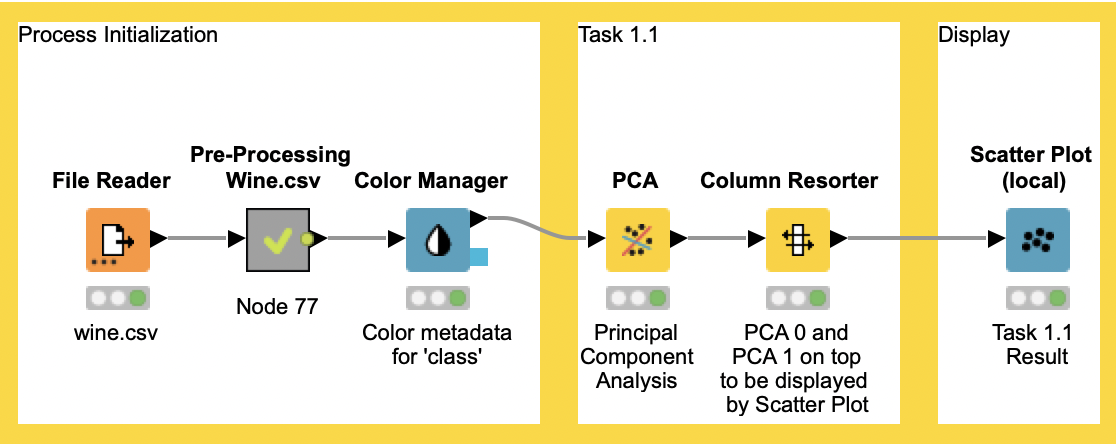
\includegraphics[scale=0.5]{res/t1/t11/t11-workflow}
			\end{center}
			\fi
			And the configurations of the nodes with descriptions are given below
			\iftrue
			\begin{figure}[H]
				\centering
				\begin{subfigure}{0.4\textwidth}
					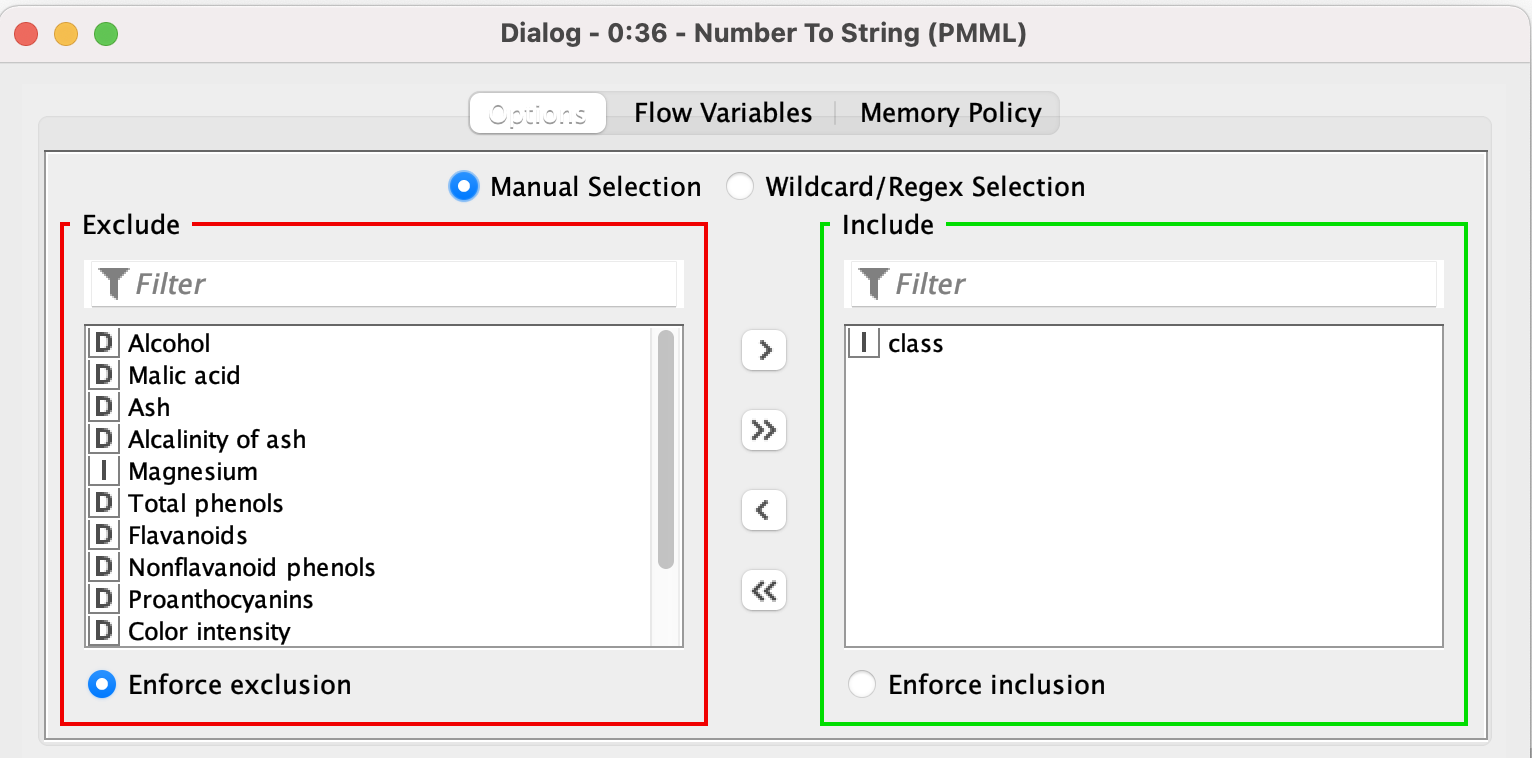
\includegraphics[width=\textwidth]{res/t1/t11/t11-number-to-cat-conf}
					\caption{Number to Category(PMML) :This node transforms the 'class' column into a categorical variable }
					\label{fig:first}
				\end{subfigure}
				\hfill
				\begin{subfigure}{0.4\textwidth}
					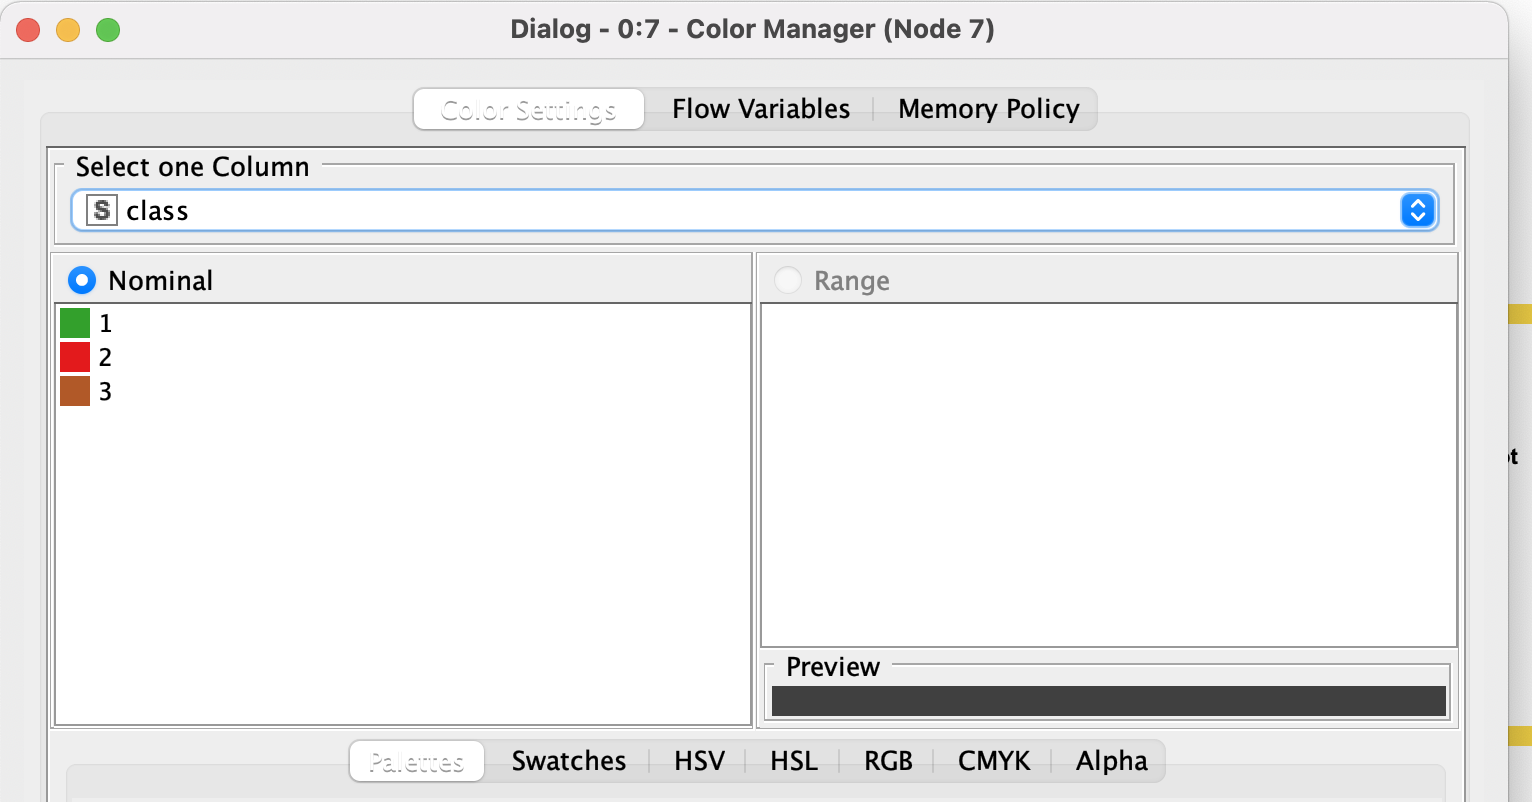
\includegraphics[width=\textwidth]{res/t1/t11/t11-color-manager-conf}
					\caption{Color Manager: Color Metadata for plot1 on class column}
					\label{fig:second}
				\end{subfigure}
				\hfill
				\begin{subfigure}{0.4\textwidth}
					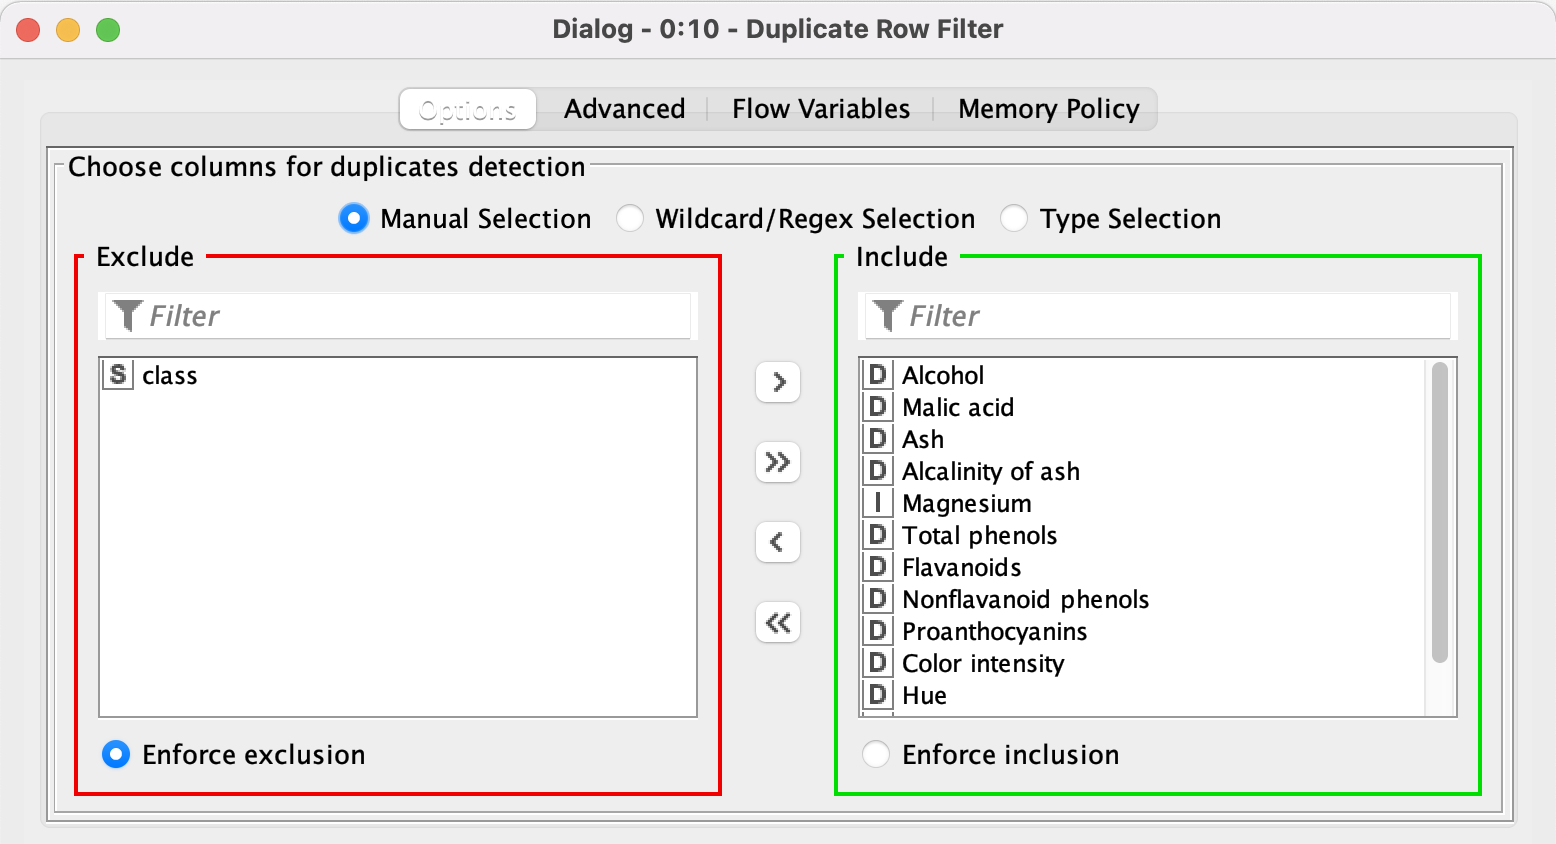
\includegraphics[width=\textwidth]{res/t1/t11/t11-duplicate-row-conf}
					\caption{Duplicate Row Filter:  Standard data clearing, worth mentioning that we exclude the 'class' variable for obvious reasons}
					\label{fig:third}
				\end{subfigure}	
				\begin{subfigure}{0.4\textwidth}
					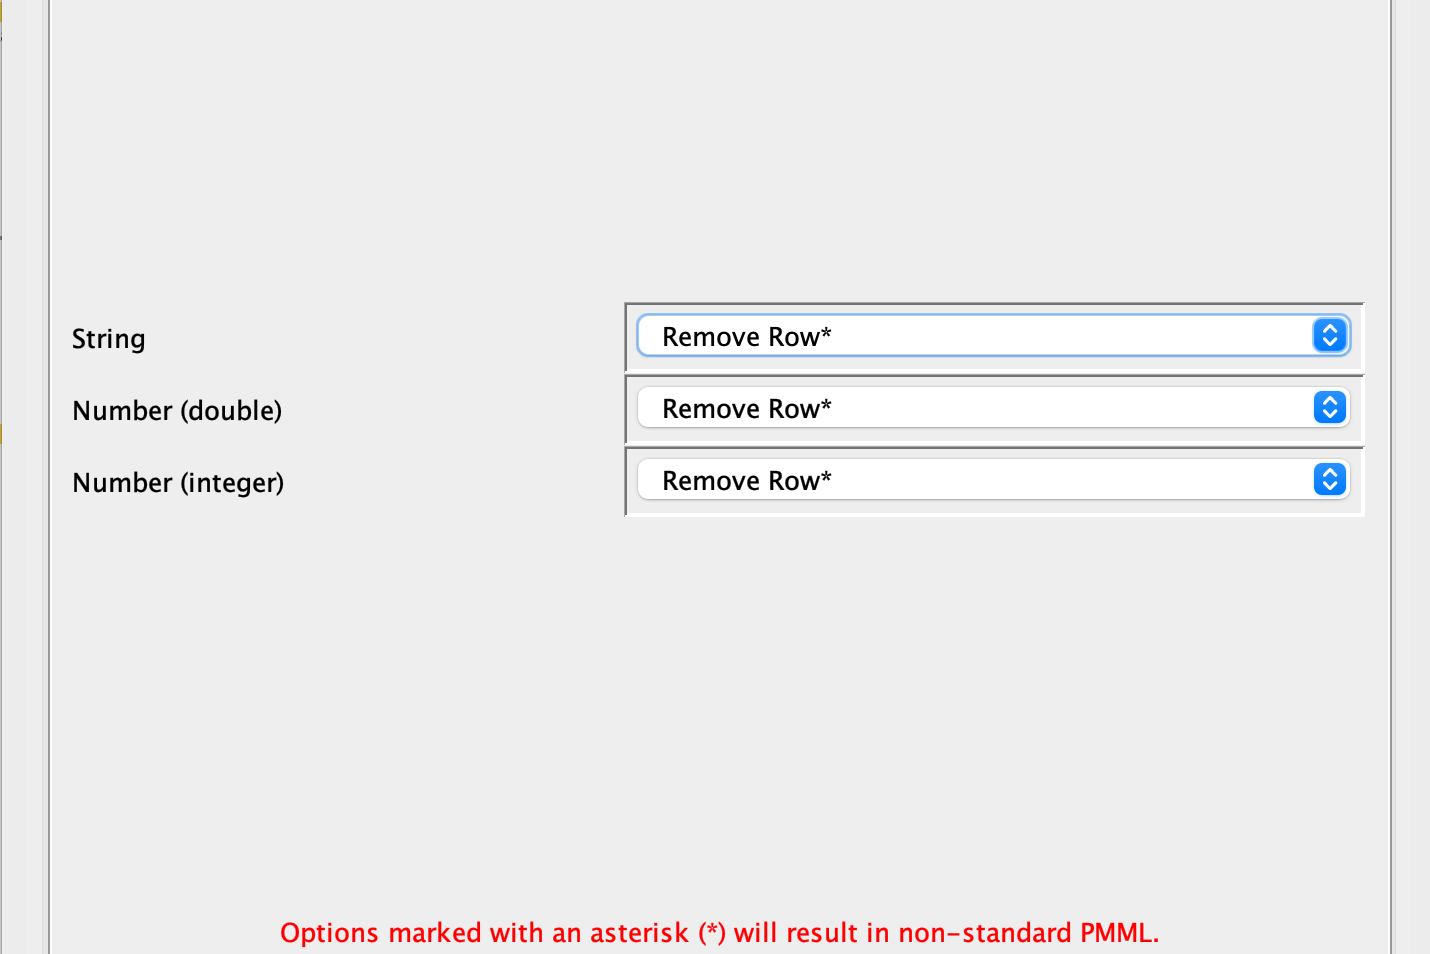
\includegraphics[scale=0.2]{res/t1/t11/t11-missing-values-conf}
					\caption{Missing Value:  Standard data clearing, removal of row in case some of the variables are empty(not observed)}
					\label{fig:first}
				\end{subfigure}
				\hfill
				\begin{subfigure}{0.4\textwidth}
					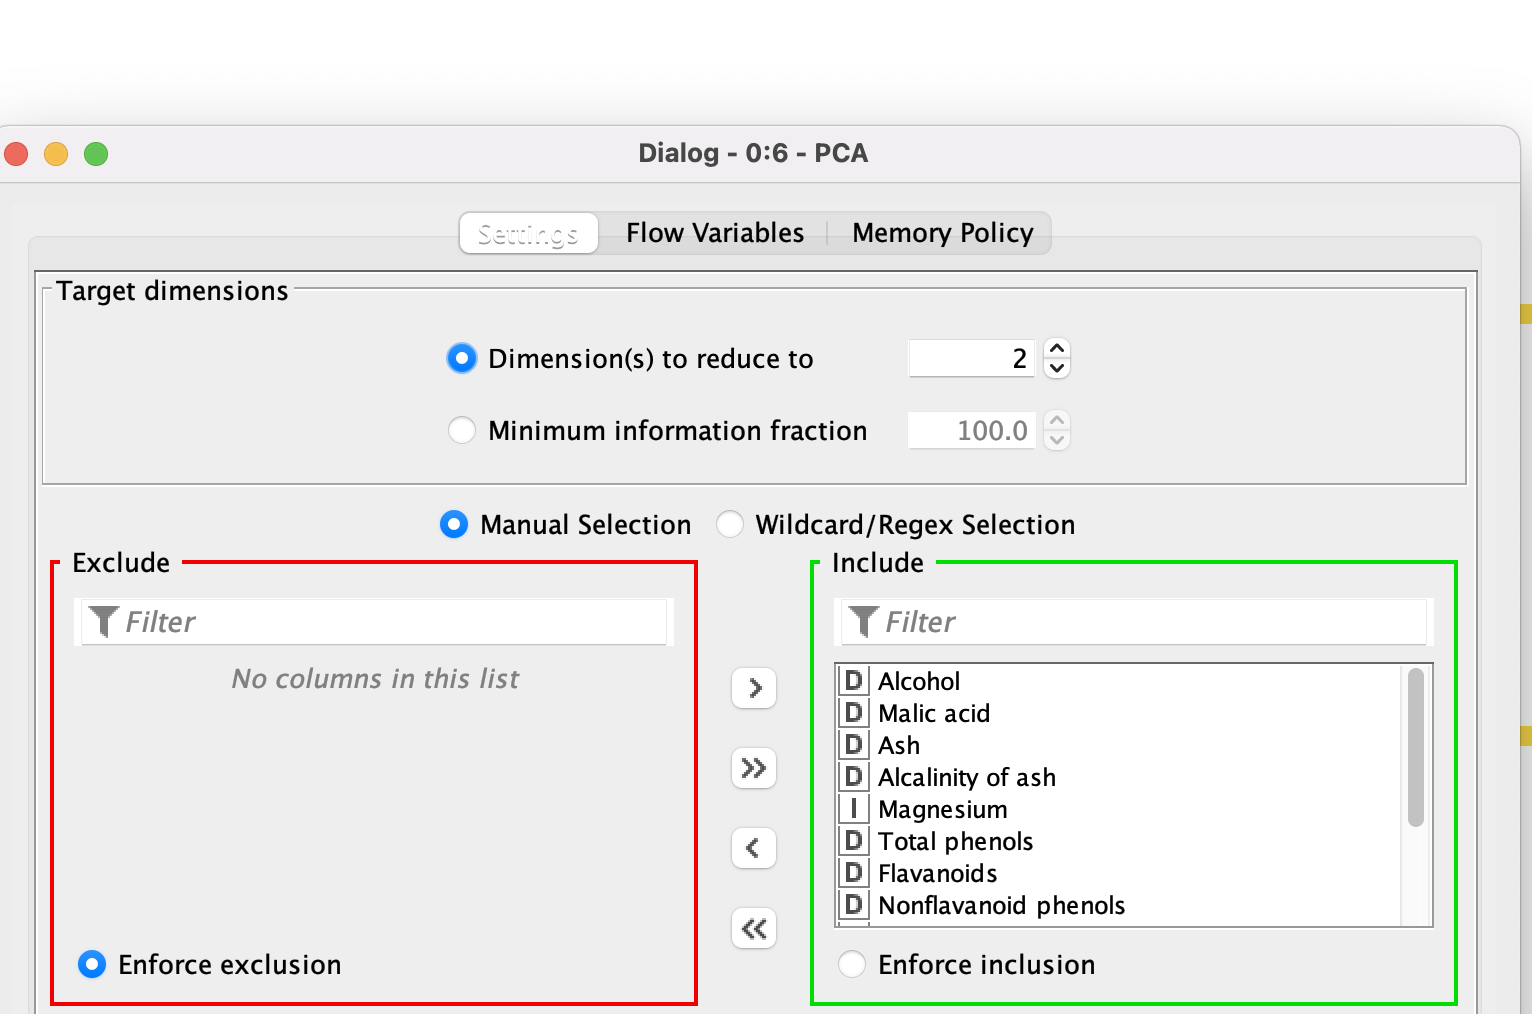
\includegraphics[width=\textwidth]{res/t1/t11/t11-PCA-conf}
					\caption{PCA: The Principal Component Analysis node, we request to reduce the dimensionality to 2, worth mentioning that, as 'class' is a string column, is automatically excluded from PCA possible collumns}
					\label{fig:second}
				\end{subfigure}
				\hfill
				\begin{subfigure}{0.4\textwidth}
					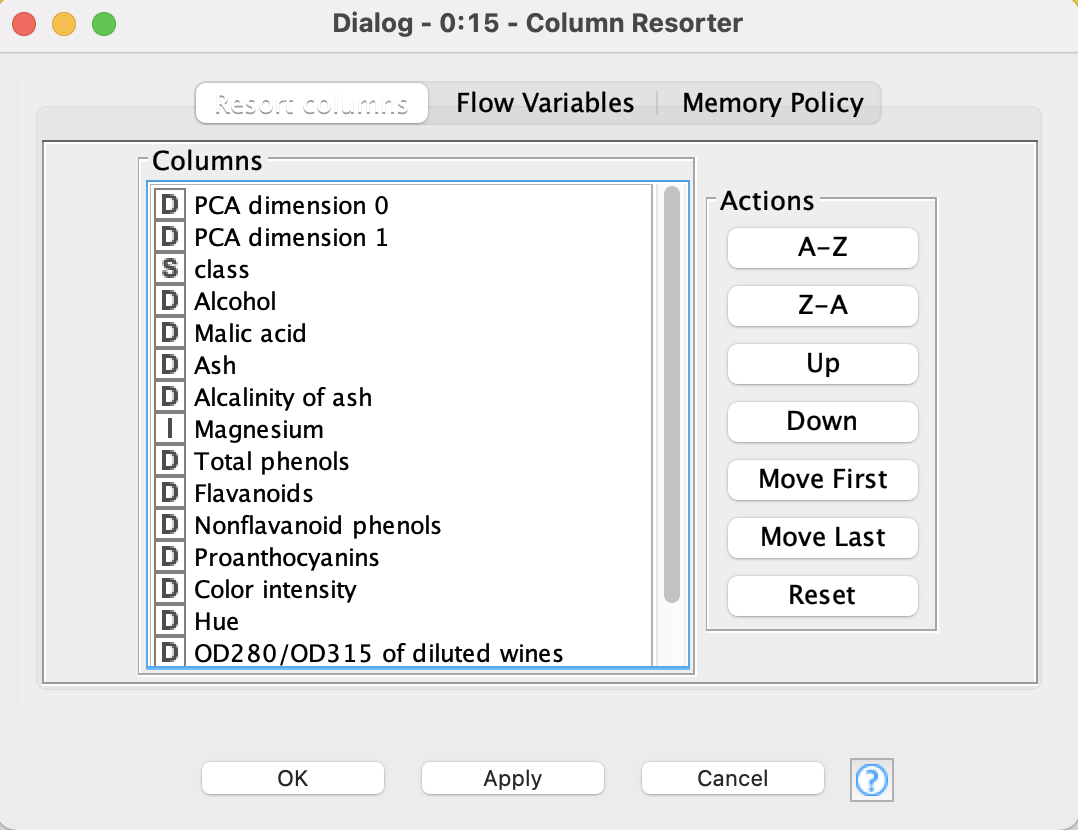
\includegraphics[width=\textwidth]{res/t1/t11/t11-column-resorter-conf}
					\caption{Column Resorter: bring first and second principal components on top(first 2 columns), to be displayed by Scatter Plot Node}
					\label{fig:third}
				\end{subfigure}	
				\label{fig:figures}
			\end{figure}
			\fi
			Finally, the plot1 is given below
			\iftrue
			\begin{center}
				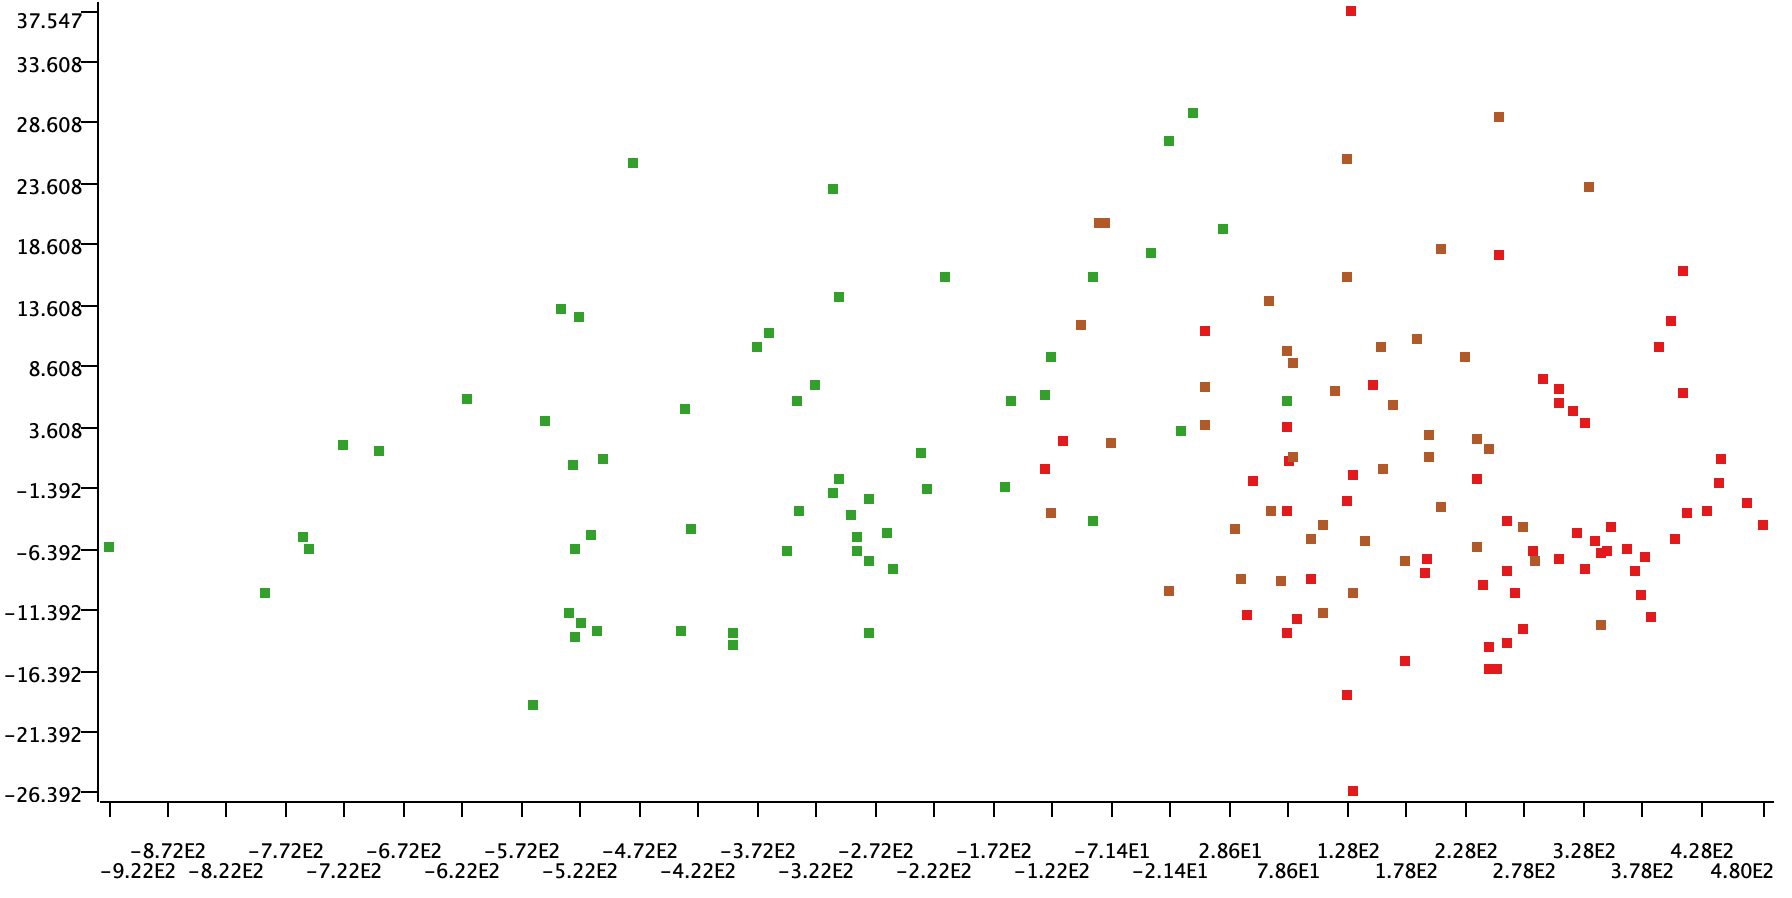
\includegraphics[scale=0.5]{res/t1/t11/t11-plot1}
			\end{center}
			\fi
		\subsection*{Task 1.2 : Generate plot2}
			The workflow to generate plot2 is given below
			\iftrue
			\begin{center}
				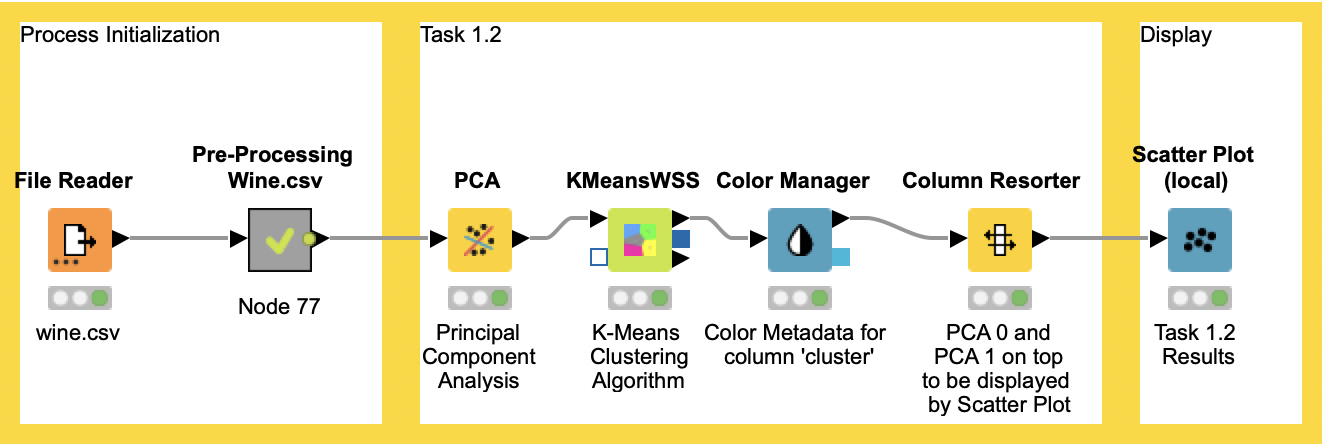
\includegraphics[scale=0.35]{res/t1/t12/t12-workflow}
			\end{center}
			\fi
			Apart from the clustering algorithm adopted(K-Means), there is no significant changes with the worflow from the previous task, please see task1.1 for an overal review of the workflow. The Newrly introduced nodes configurations, as well as the descriptions are given below
			
			\iftrue
			\begin{figure}[H]
				\centering
				\begin{subfigure}{0.4\textwidth}
					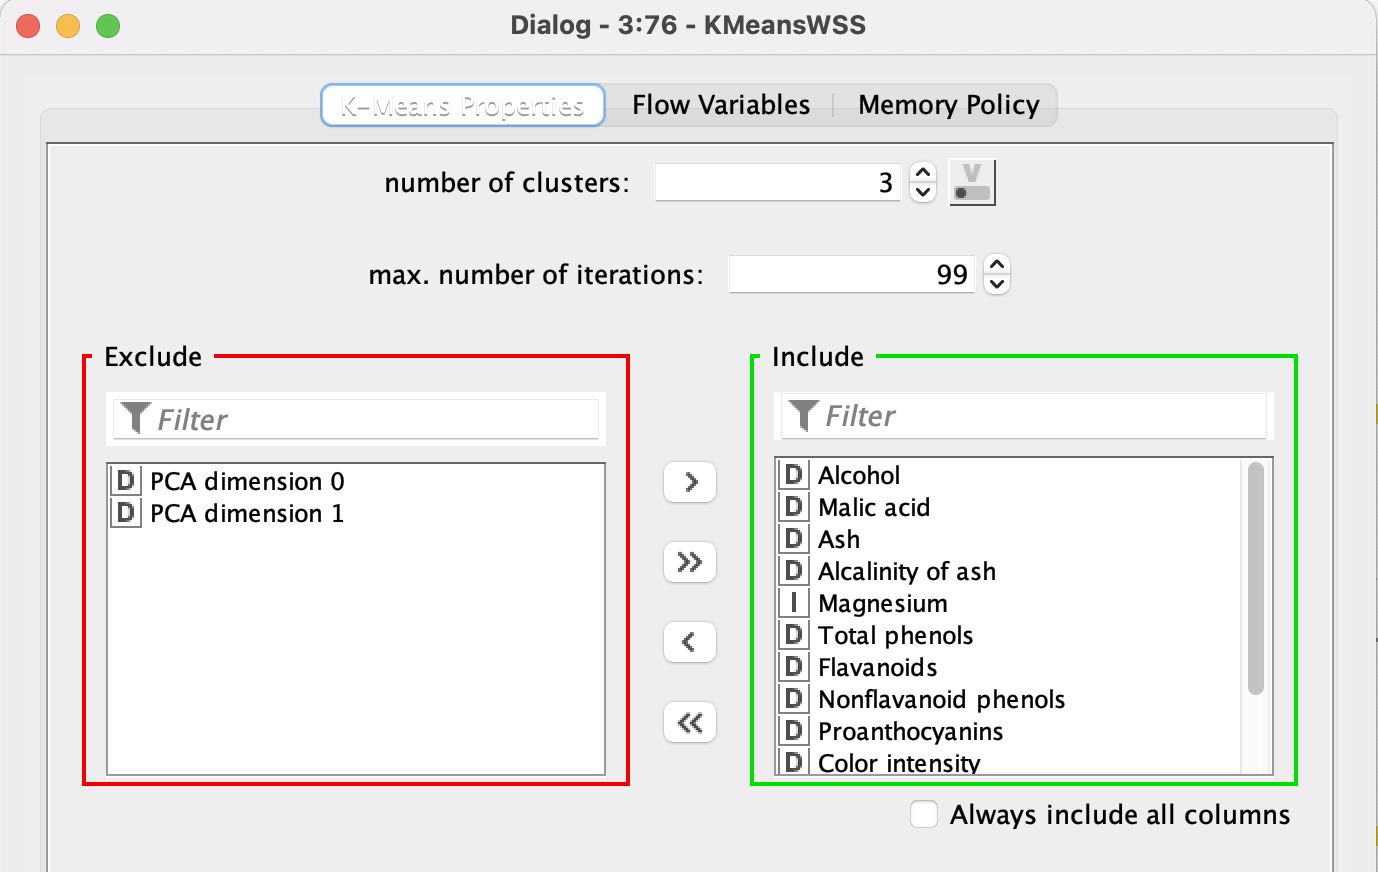
\includegraphics[width=\textwidth]{res/t1/t12/t12-kmeans-wss-conf}
					\caption{KMeansWSS : this node implements our clustering algorithm of choice, the exact inner-workings to be explained on the next paragraph. A noteworthy configuration is the exclusion of PCA dimensions from the clustering process}
					\label{fig:first}
				\end{subfigure}
				\hfill
				\begin{subfigure}{0.4\textwidth}
					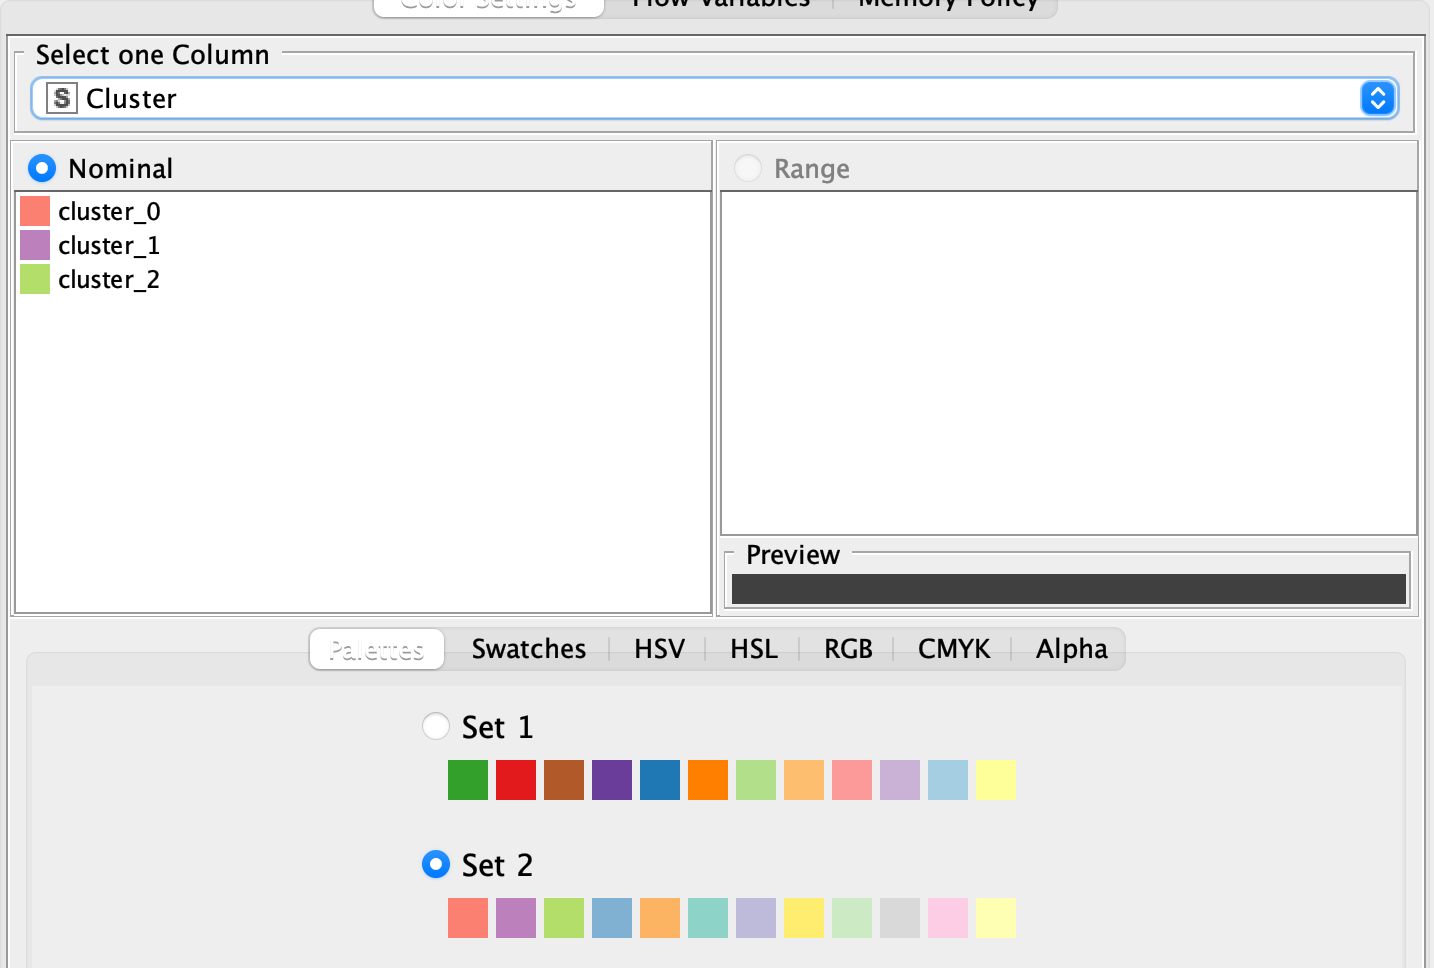
\includegraphics[width=\textwidth]{res/t1/t12/t12-color-manager-conf}
					\caption{Color Manager: After KMeans finishes, we add colour metadata to our 'cluster' column, generated by the aforementioned KMeansWSS Node, to be displayed by the Scatter Plot node. The colour palette is different from the colour palette chosen on Task1.1}
					\label{fig:second}
				\end{subfigure}
				\hfill
			\end{figure}
			\fi
			Finally, the plot2 is given below
			\iftrue
			\begin{center}
				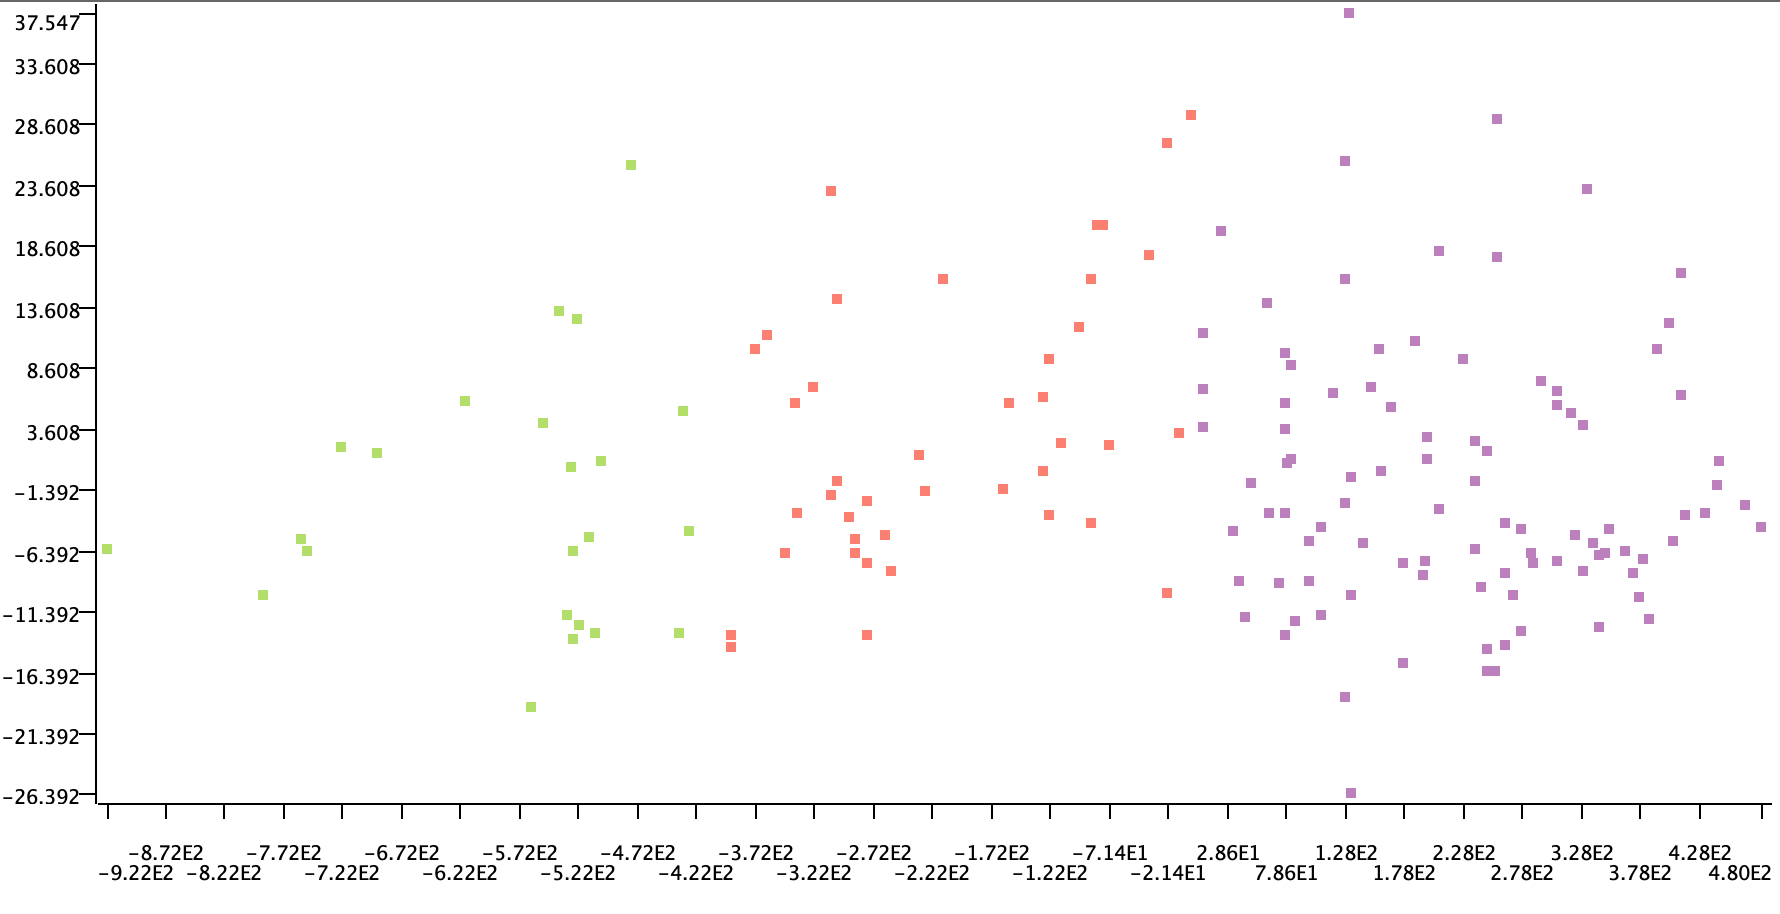
\includegraphics[scale=0.5]{res/t1/t12/t12-plot2}
			\end{center}
			\fi
			\subsubsection{K-Means clustering algorithm}
				The standard Lorem Ipsum passage, used since the 1500s
				
				"Lorem ipsum dolor sit amet, consectetur adipiscing elit, sed do eiusmod tempor incididunt ut labore et dolore magna aliqua. Ut enim ad minim veniam, quis nostrud exercitation ullamco laboris nisi ut aliquip ex ea commodo consequat. Duis aute irure dolor in reprehenderit in voluptate velit esse cillum dolore eu fugiat nulla pariatur. Excepteur sint occaecat cupidatat non proident, sunt in culpa qui officia deserunt mollit anim id est laborum."
				Section 1.10.32 of "de Finibus Bonorum et Malorum", written by Cicero in 45 BC
				
				 
		 \subsection*{Task 1.3 : Compare plot1 and plot2}
			The main point of interest in the figures above, is the fact that, the clustering algorithm(K-Means, k=3) failed to appropriately partition the data, and recognise the classes provided by the dataset, This phenomenon can be explained due to the absence of the standardization process, something that will be explained in the next Task. The exact scale of the problem cannot be appropriately assessed with only those two plots though, we will need to examine the distribution of the classes in each cluster, something that will be done on the next task(Task 1.4)
		
		 \subsection*{Task 1.4 : plot3a,plot3b,plot3c}
			
			
			The workflow to generate the requested plots is given below
			\iftrue
			\begin{center}
				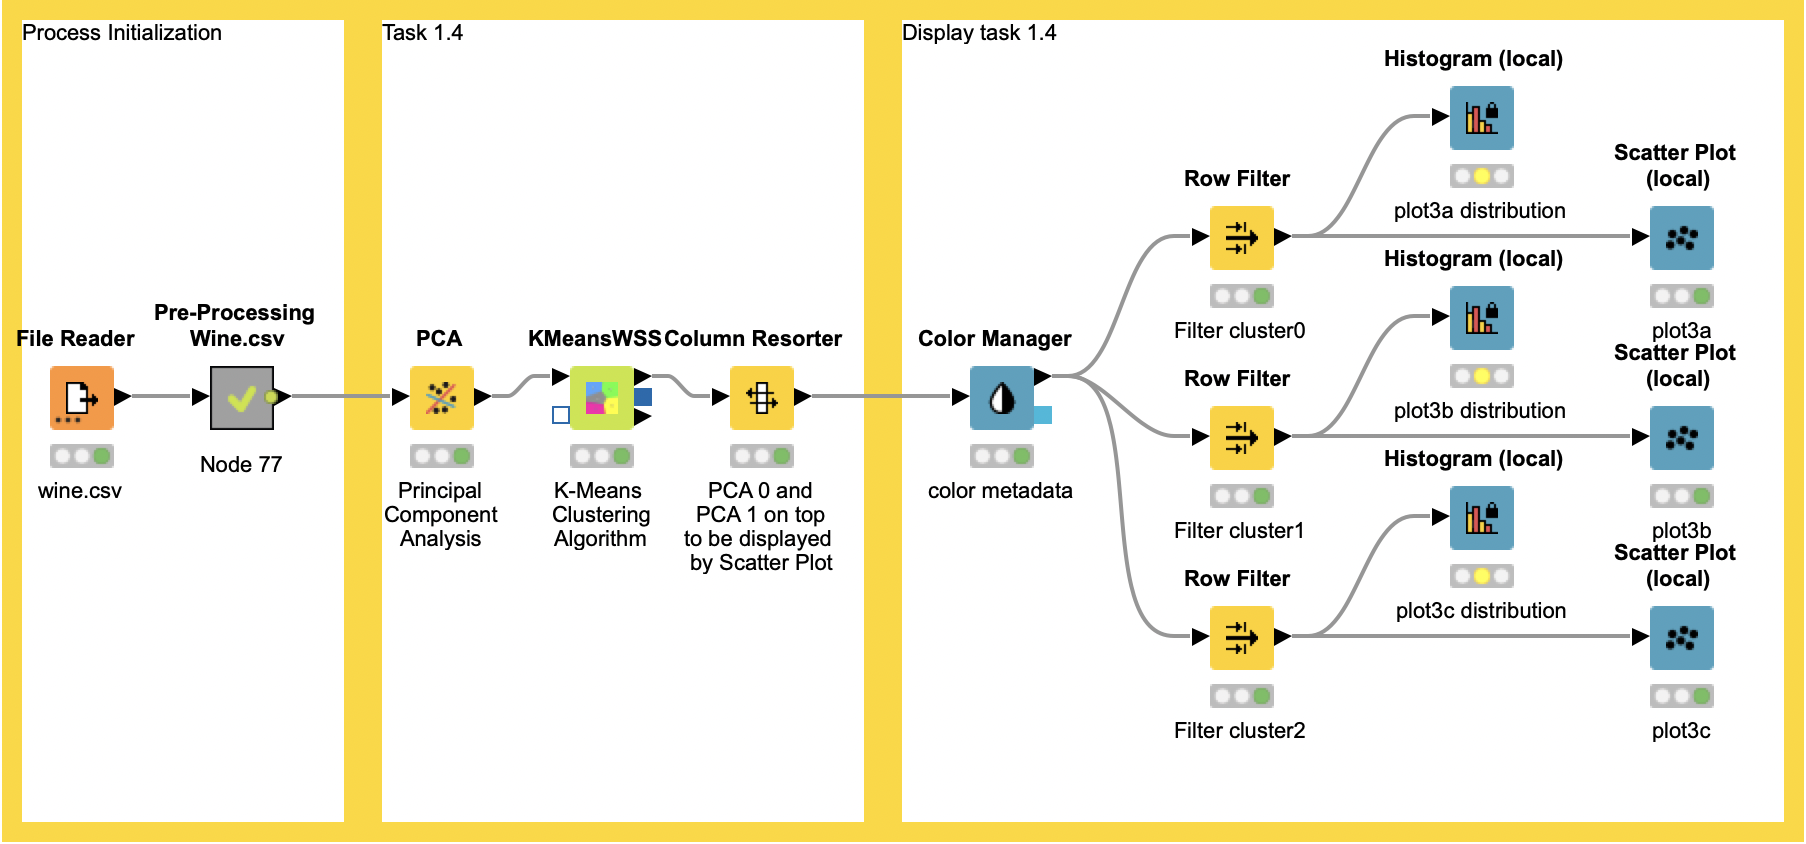
\includegraphics[scale=0.25]{res/t1/t14/t14-workflow}
			\end{center}
			\fi
			The majority of the workflow is identical to workflows of task1.1 and task1.2, so please refer to those tasks for a detailed explanations of those nodes. The major difference is on the display section. There, we use 3 row filters(one per cluster) to filter the datapoints that were assigned on each cluster. Hence in the first plot, we have all the datapoints assigned to cluster0 and vice versa. The node configurations with the nessesary filters are given below
			\iftrue
			\begin{figure}[H]
				\centering
				\begin{subfigure}{0.4\textwidth}
					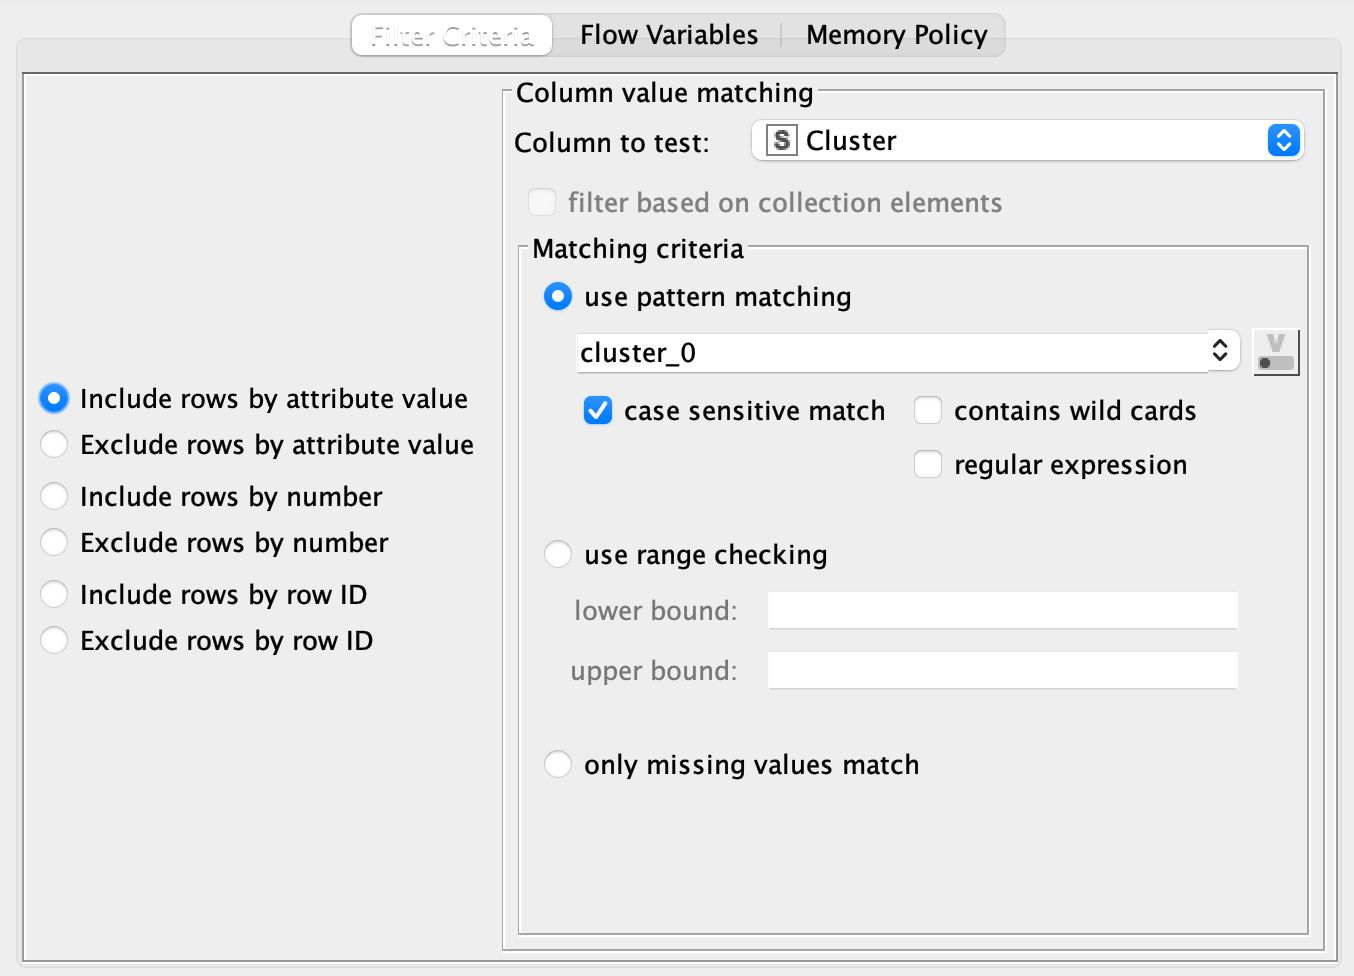
\includegraphics[width=\textwidth]{res/t1/t14/t14-row-filter-1-conf}
					\caption{Row filter: cluster0 filter}
					\label{fig:first}
				\end{subfigure}
				\hfill
				\begin{subfigure}{0.4\textwidth}
					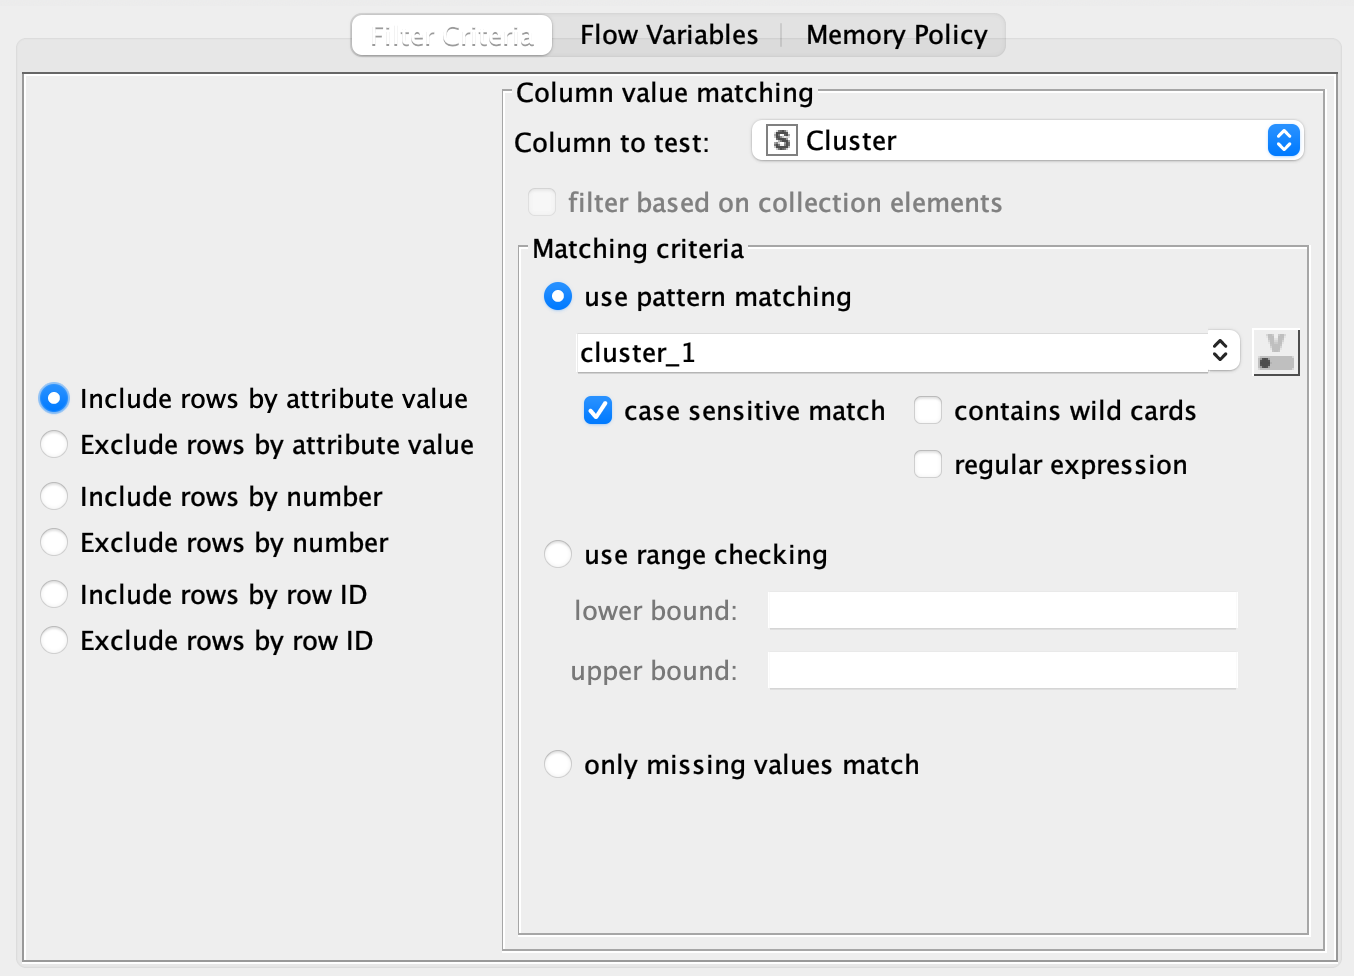
\includegraphics[width=\textwidth]{res/t1/t14/t14-row-filter-2-conf}
					\caption{Row filter: cluster1 filter}
					\label{fig:second}
				\end{subfigure}
				\hfill
				\begin{subfigure}{0.4\textwidth}
					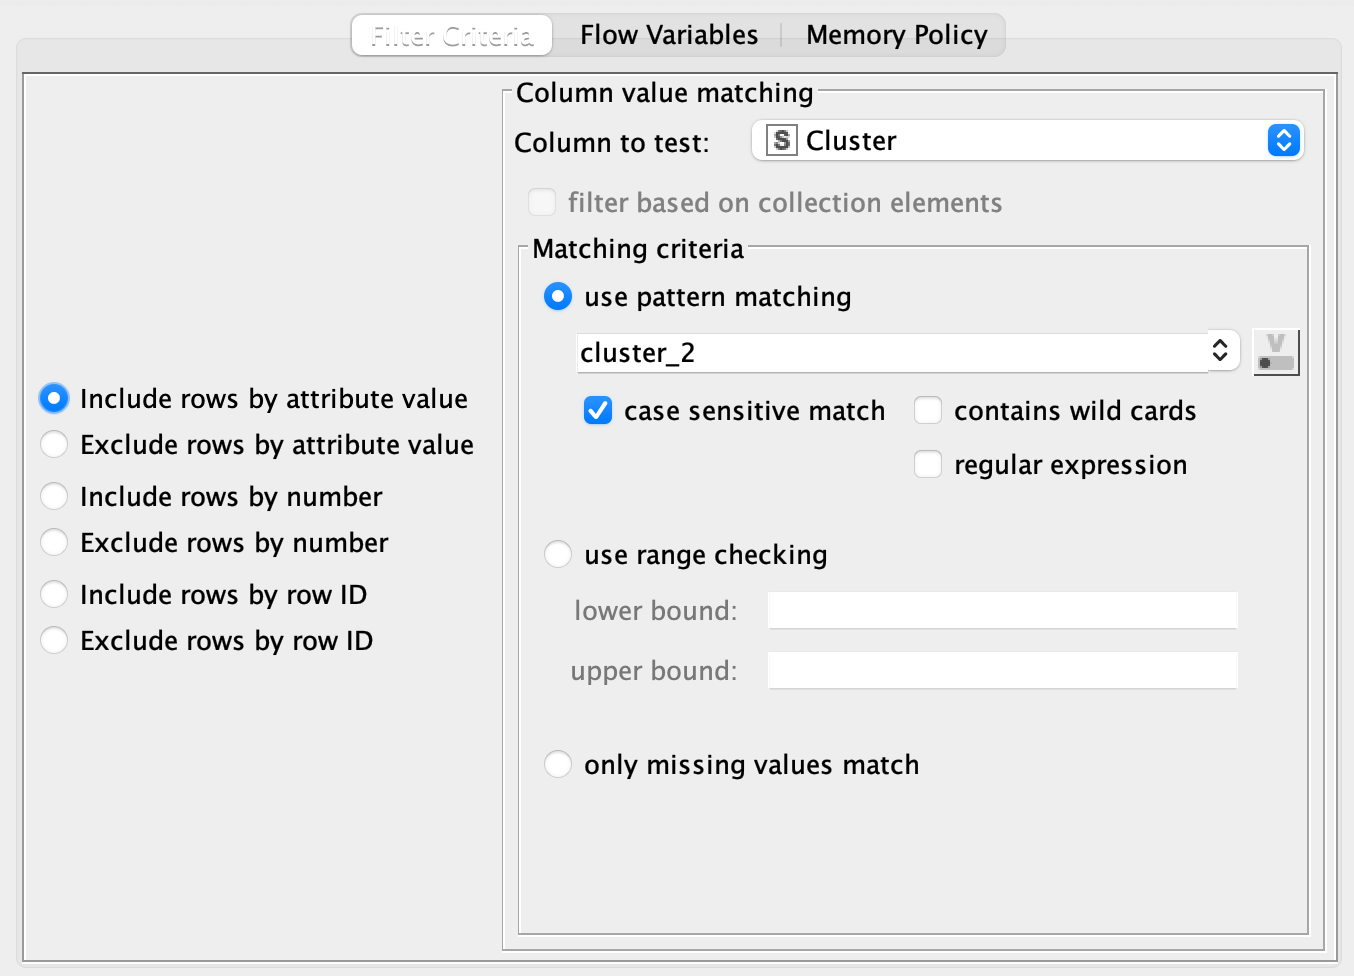
\includegraphics[width=\textwidth]{res/t1/t14/t14-row-filter-3-conf}
					\caption{Row filter: cluster2 filter}
					\label{fig:third}
				\end{subfigure}	
				\label{fig:figures}
			\end{figure}
			\fi
			
			
			Finally, the generated plots are given in the next figure.
			\iftrue
			 \begin{figure}[H]
			 	\centering
			 	\begin{subfigure}{0.4\textwidth}
			 		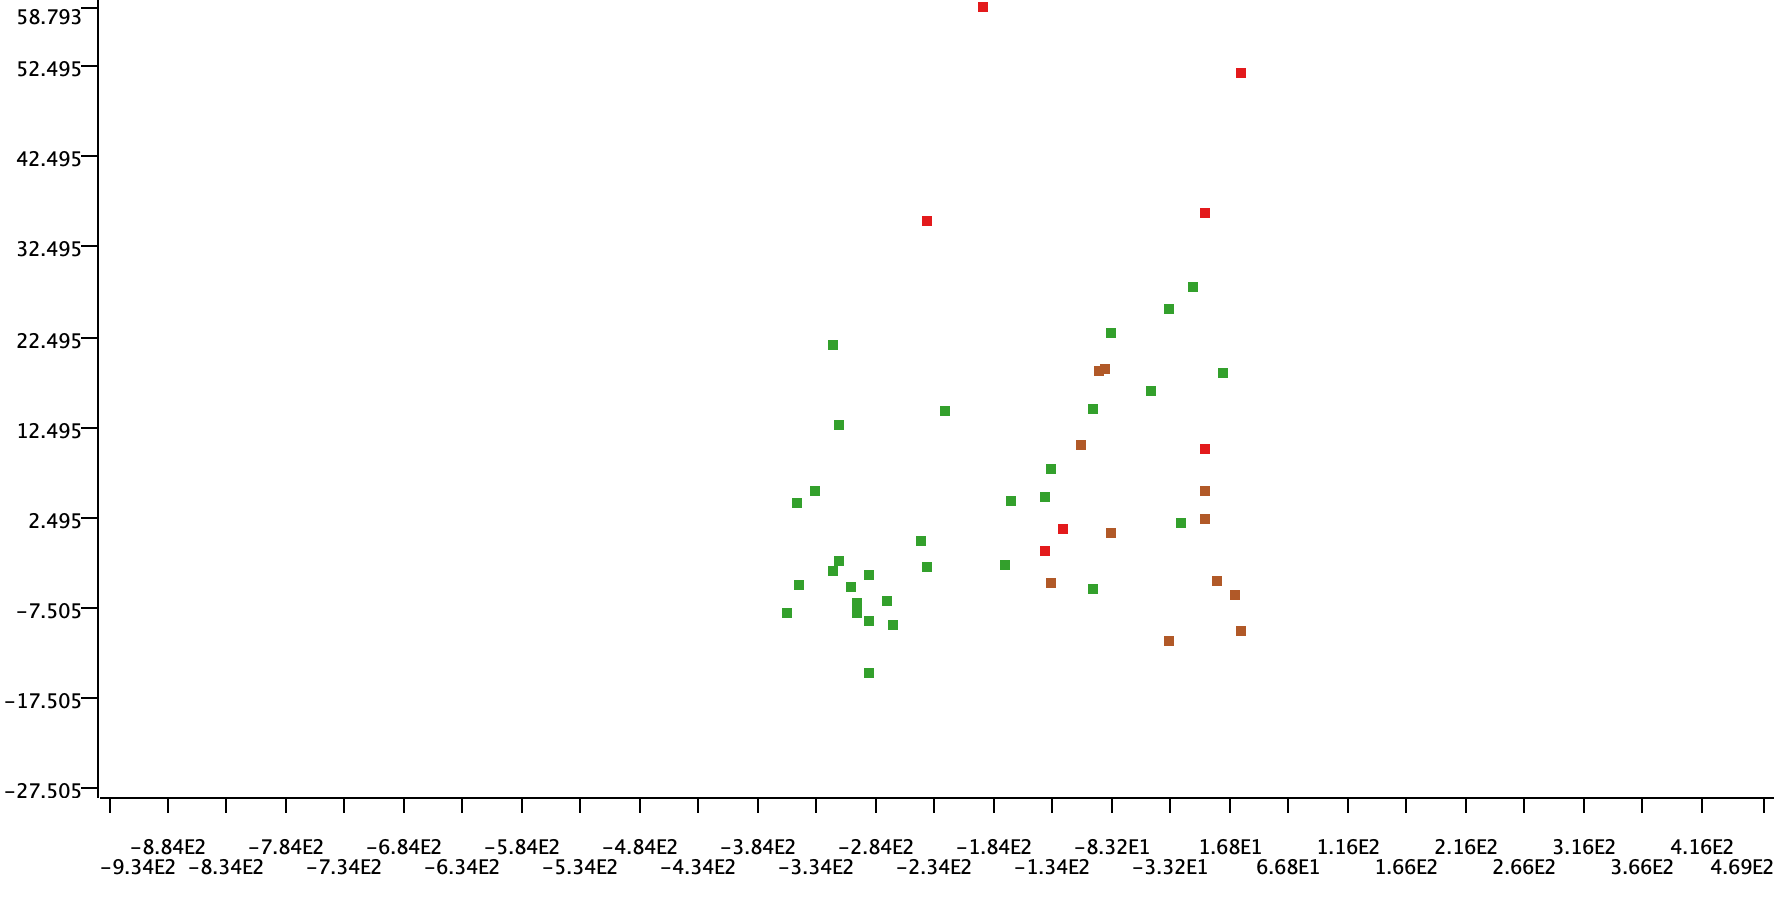
\includegraphics[width=\textwidth]{res/t1/t14/t14-plota}
			 		\caption{plot3a}
			 		\label{fig:first}
			 	\end{subfigure}
			 	\hfill
			 	\begin{subfigure}{0.4\textwidth}
			 		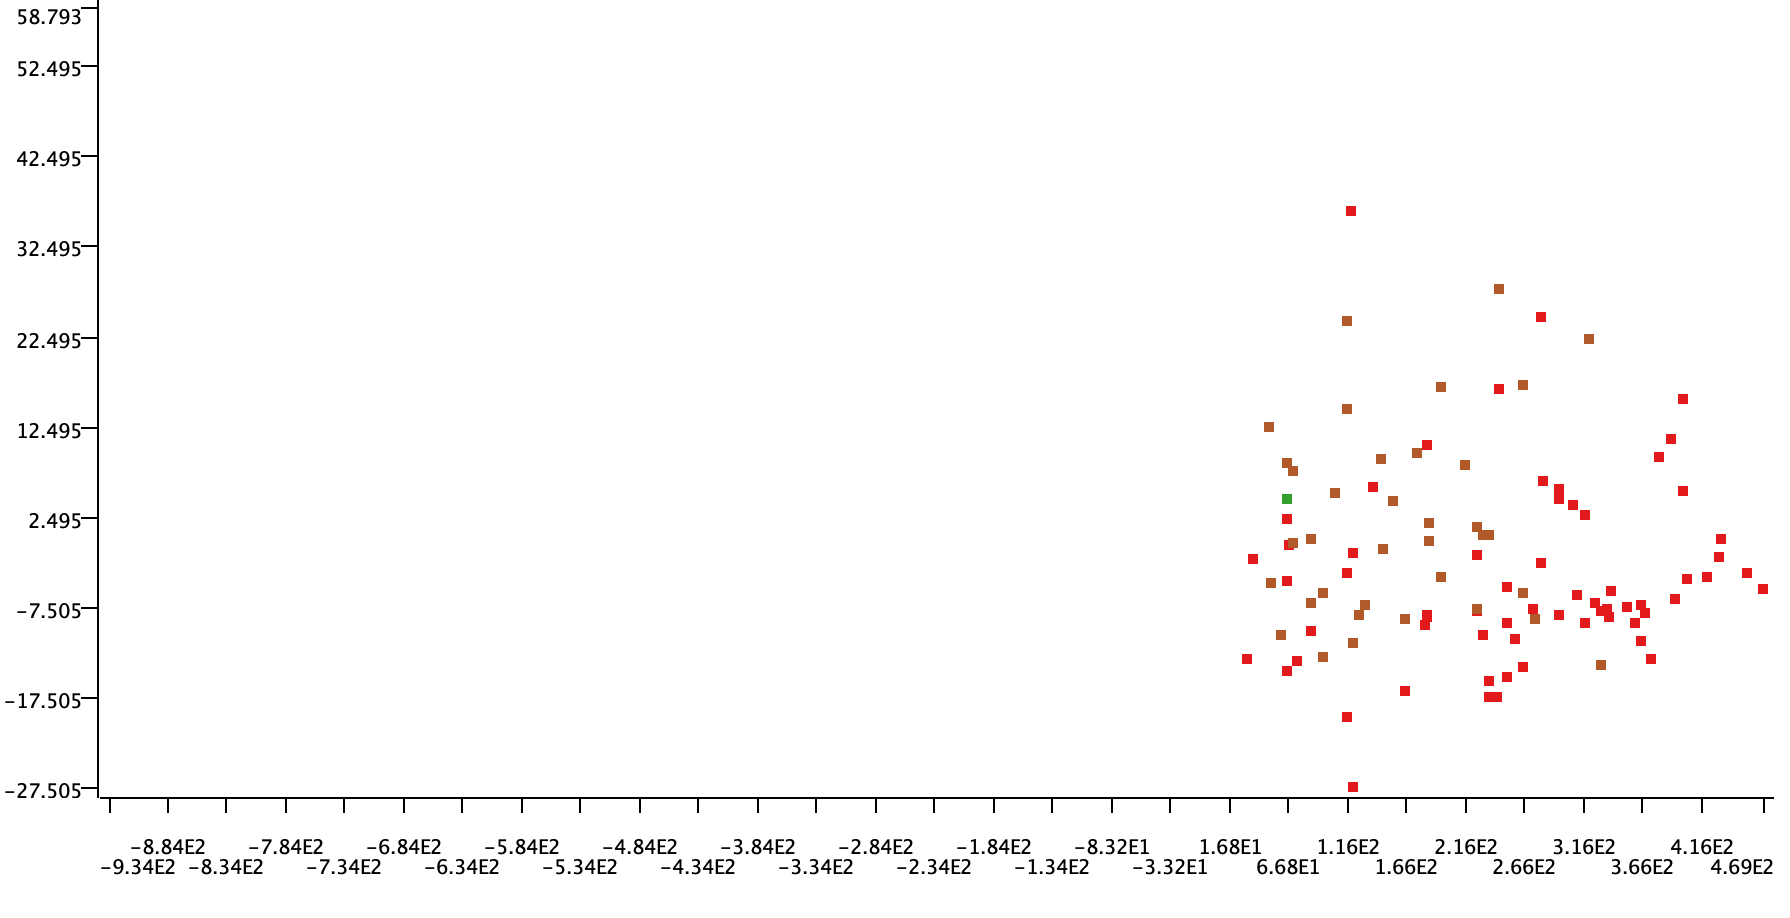
\includegraphics[width=\textwidth]{res/t1/t14/t14-plotb}
			 		\caption{plot3b}
			 		\label{fig:second}
			 	\end{subfigure}
			 	\hfill
			 	\begin{subfigure}{0.4\textwidth}
			 		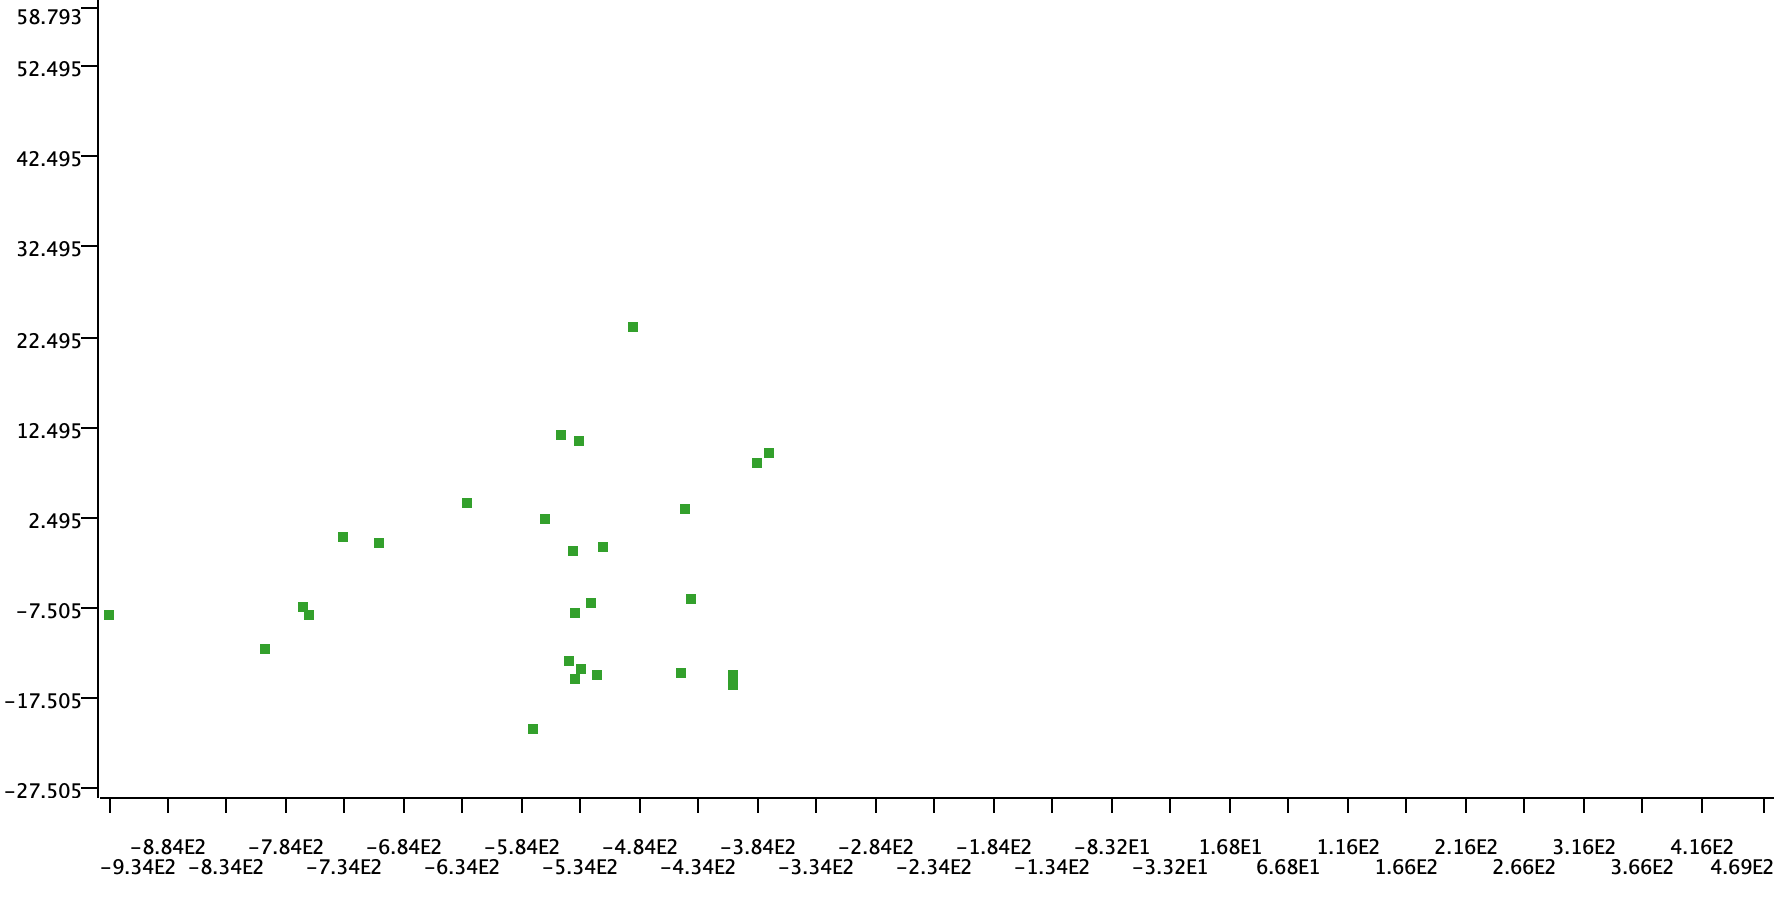
\includegraphics[width=\textwidth]{res/t1/t14/t14-plotc}
			 		\caption{plot3c}
			 		\label{fig:third}
			 	\end{subfigure}
			 	\label{fig:figures} 
			 \end{figure}
		 	\fi
			It becomes apparent that the clusters generated are composing an meaningless clustering solution. Under ideal circumstances, each cluster will had a vast majority of each of the classes, with some to none variation due to outliers or errors, Using histograms we can visualize the extend of the issue 
			\iftrue
			\begin{figure}[H]
				\centering
				\begin{subfigure}{0.4\textwidth}
			 		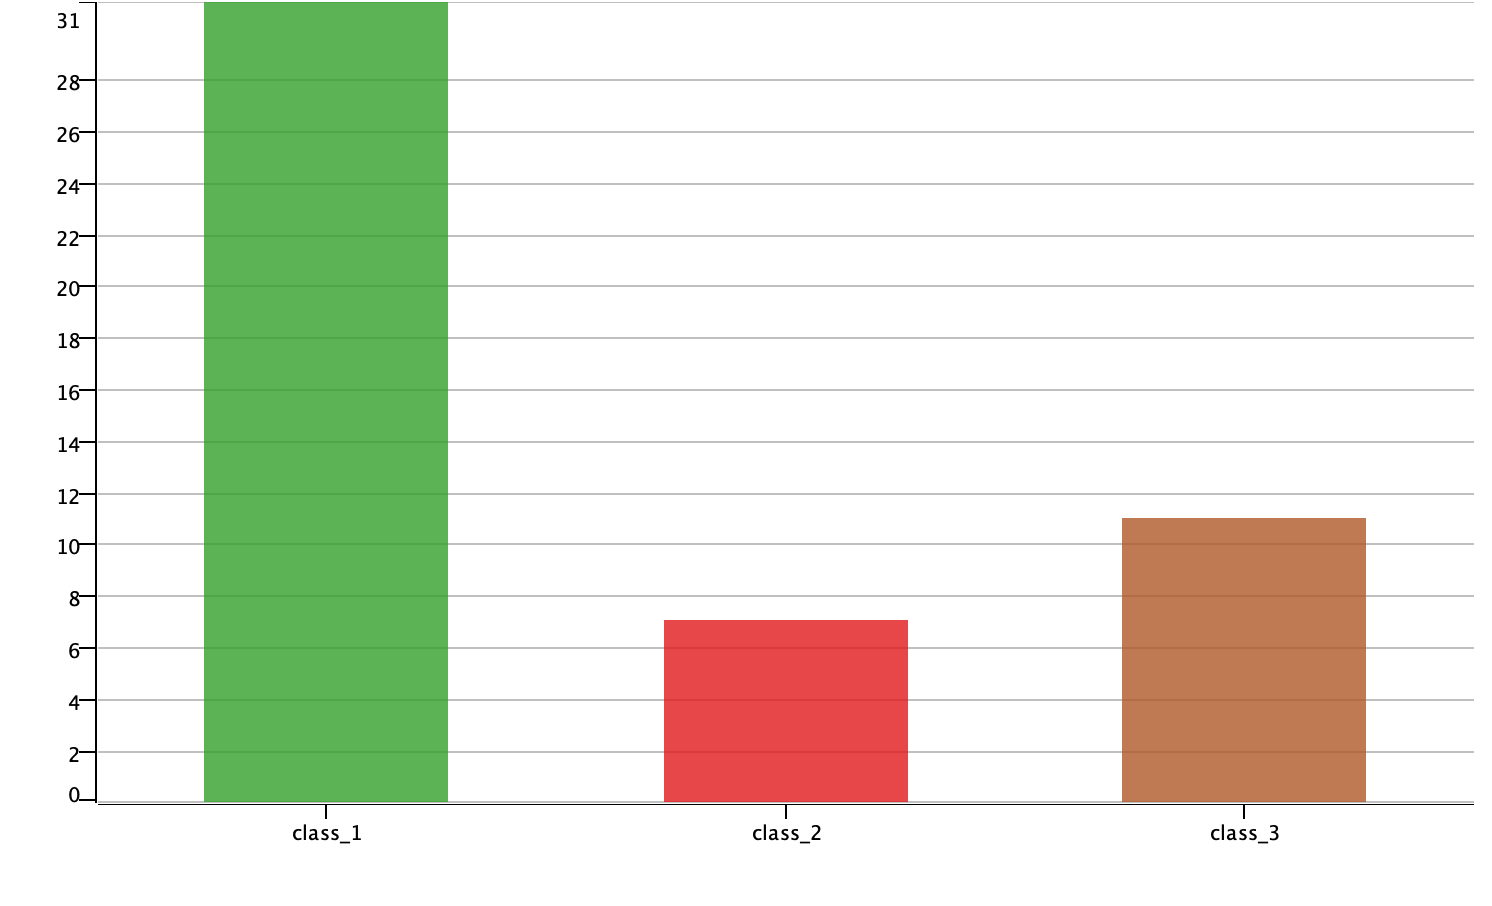
\includegraphics[width=\textwidth]{res/t1/t14/t14-plota-dist}
					\caption{plot3a distribution}
					\label{fig:first}
				\end{subfigure}
				\hfill
				\begin{subfigure}{0.4\textwidth}
			 		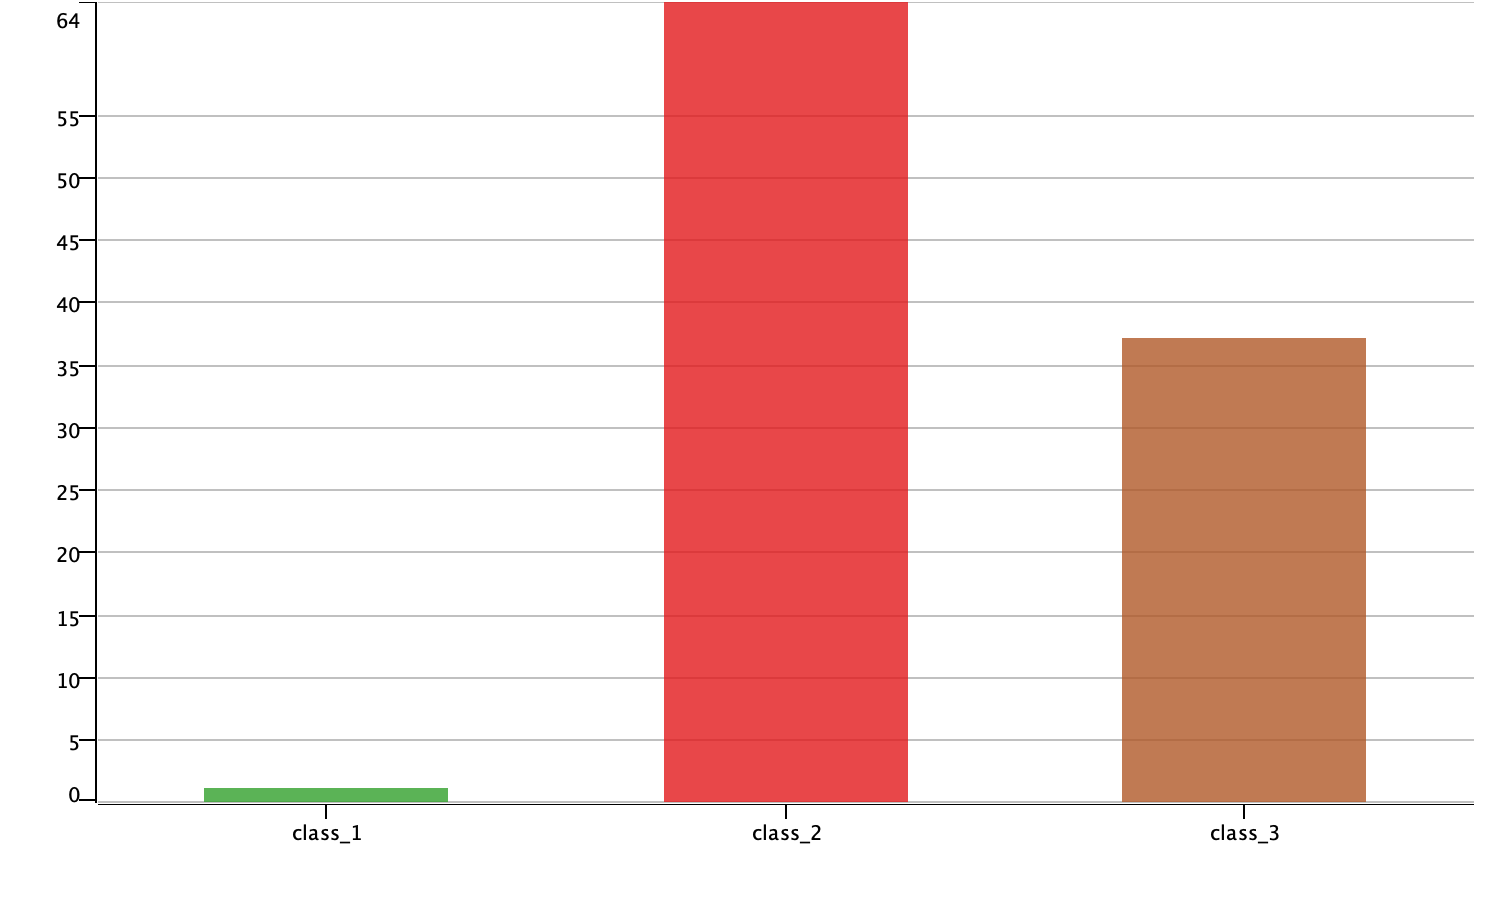
\includegraphics[width=\textwidth]{res/t1/t14/t14-plotb-dist}
					\caption{plot3b distribution}
					\label{fig:second}
				\end{subfigure}
				\hfill
				\begin{subfigure}{0.4\textwidth}
			 		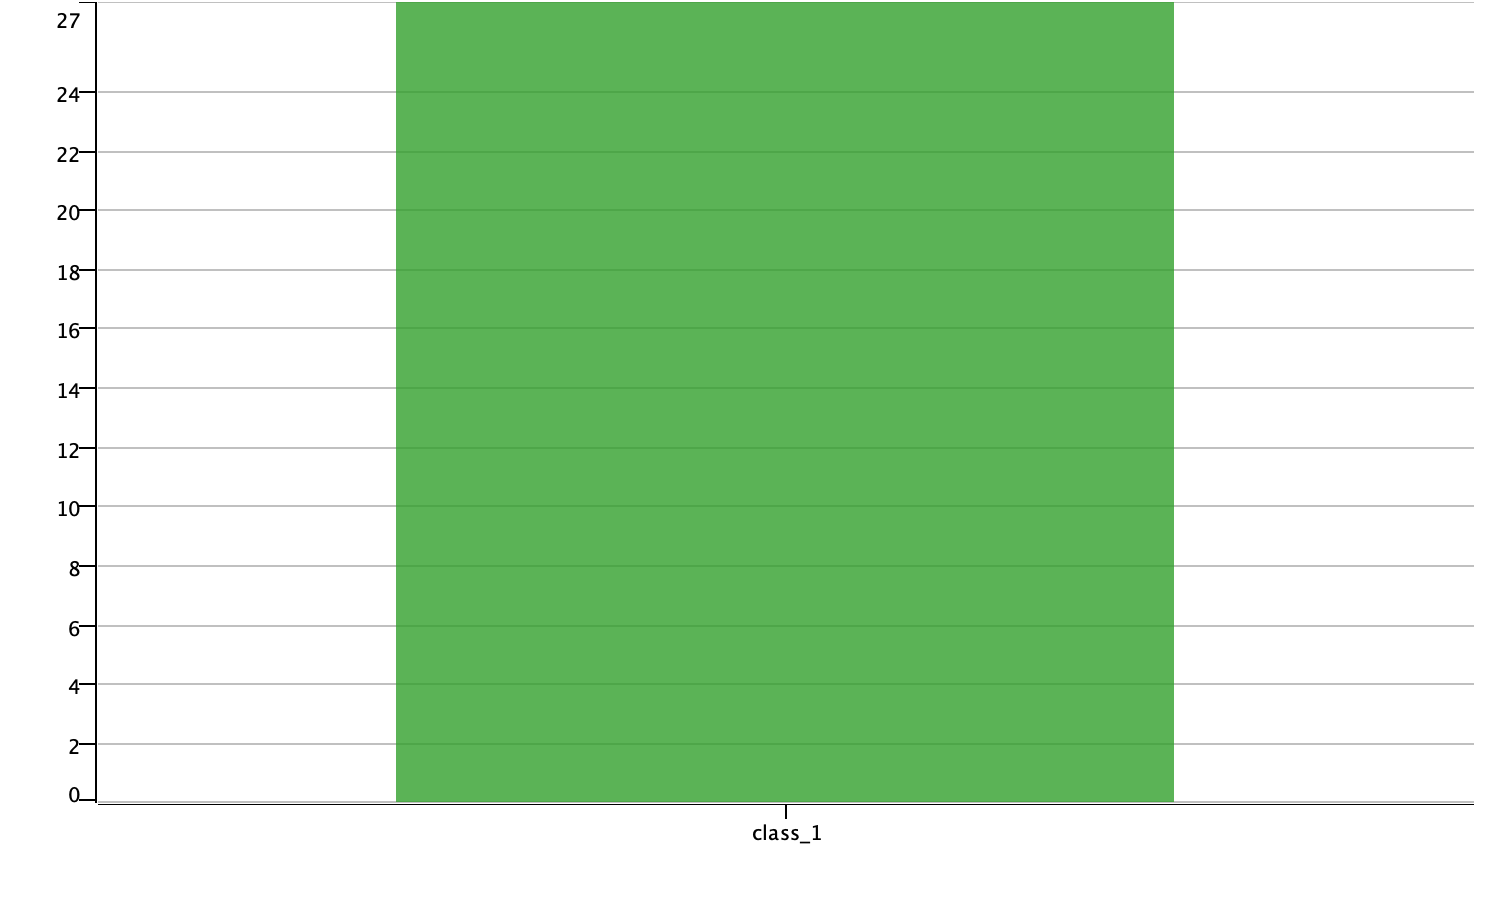
\includegraphics[width=\textwidth]{res/t1/t14/t14-plotc-dist}
					\caption{plot3c distribution}
					\label{fig:third}
				\end{subfigure}	
				\label{fig:figures}
			\end{figure}
			\fi
			 This is the result of the lack of a normalization/standarization process, something that we will explain on the next task.
		\subsection*{Task 1.5 : Cluster Validity Measure}
			For our cluster validity measure, we will explain and intepret WSS (Within cluster sum of squares) and BSS (Between cluster sum of squares). The workflow for generating the cluster validity measures is given below
			\iftrue
			\begin{center}
				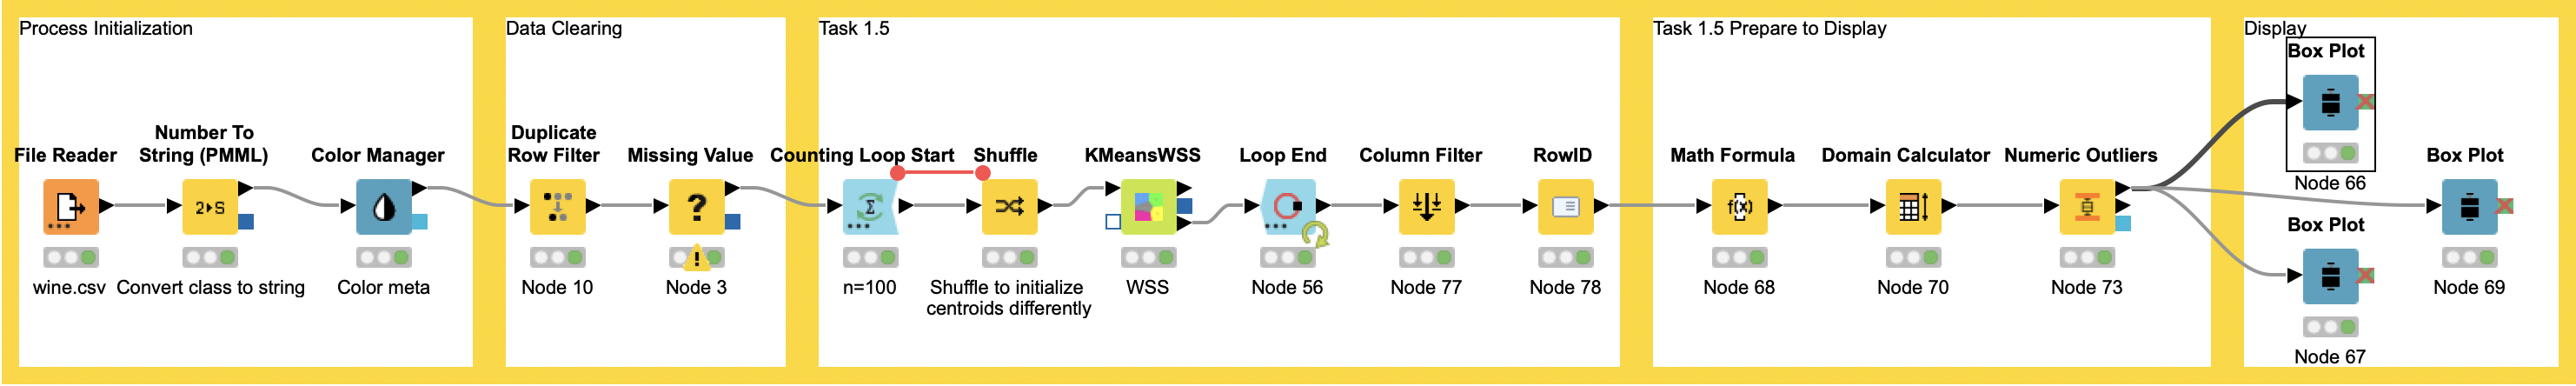
\includegraphics[scale=0.25]{res/t1/t15/t15-workflow}
			\end{center}
			\fi
			The majority of the workflow is identical to workflows of task1.1 to task1.4, so please refer to those tasks for a detailed explanations of those nodes. The Major Difference is on the repeat process and on the intepretation proccess. The newrly introduced nodes configurations are given below, along with a short explanation
			\iftrue
			\begin{figure}[H]
				\centering
				\begin{subfigure}{0.4\textwidth}
					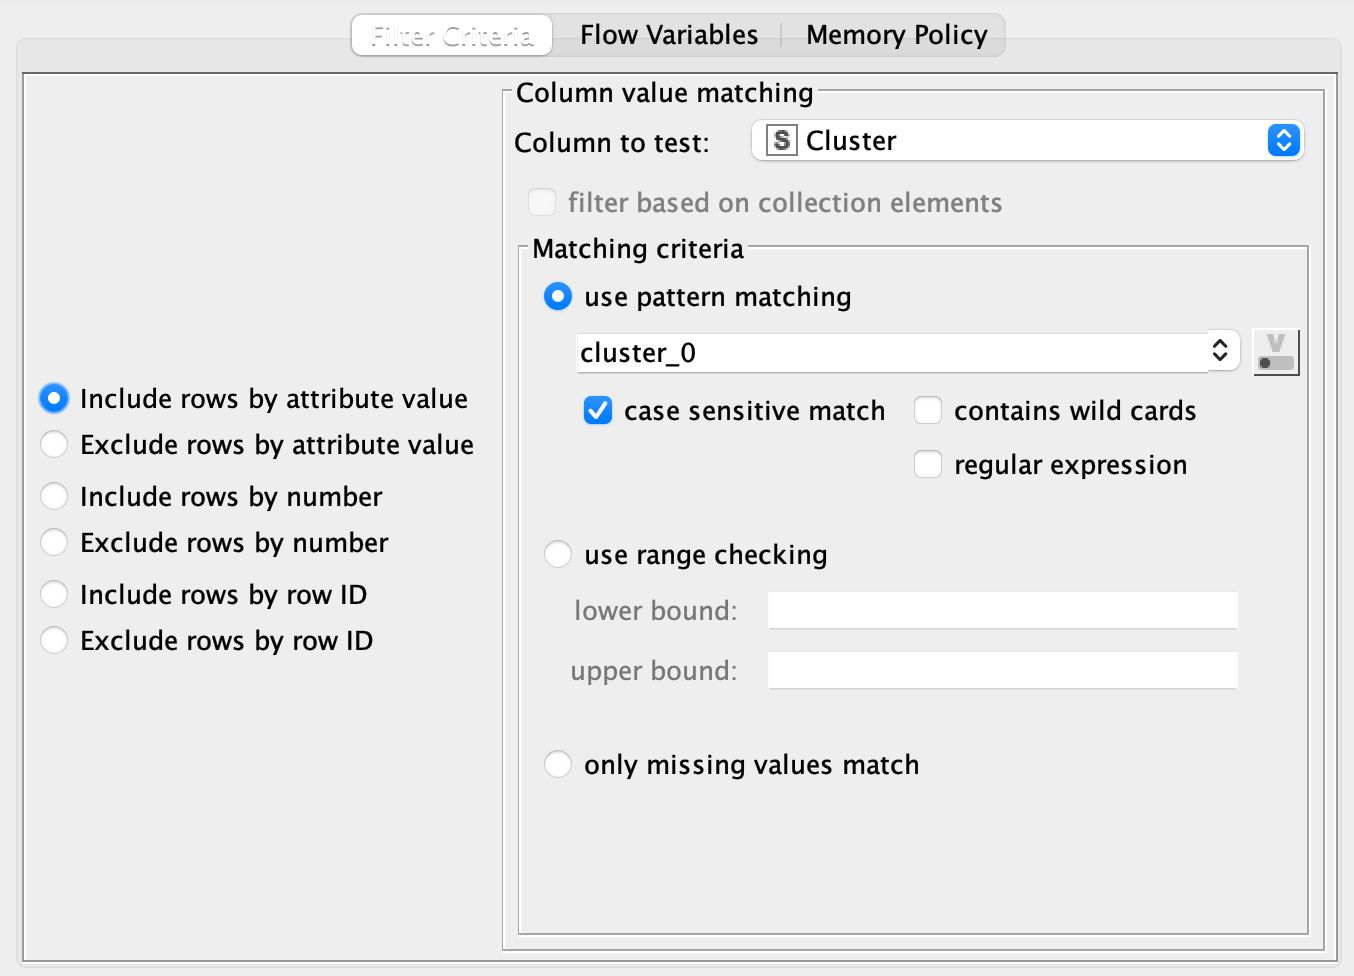
\includegraphics[width=\textwidth]{res/t1/t14/t14-row-filter-1-conf}
					\caption{Number to Category(PMML)}
					\label{fig:first}
				\end{subfigure}
				\hfill
				\begin{subfigure}{0.4\textwidth}
					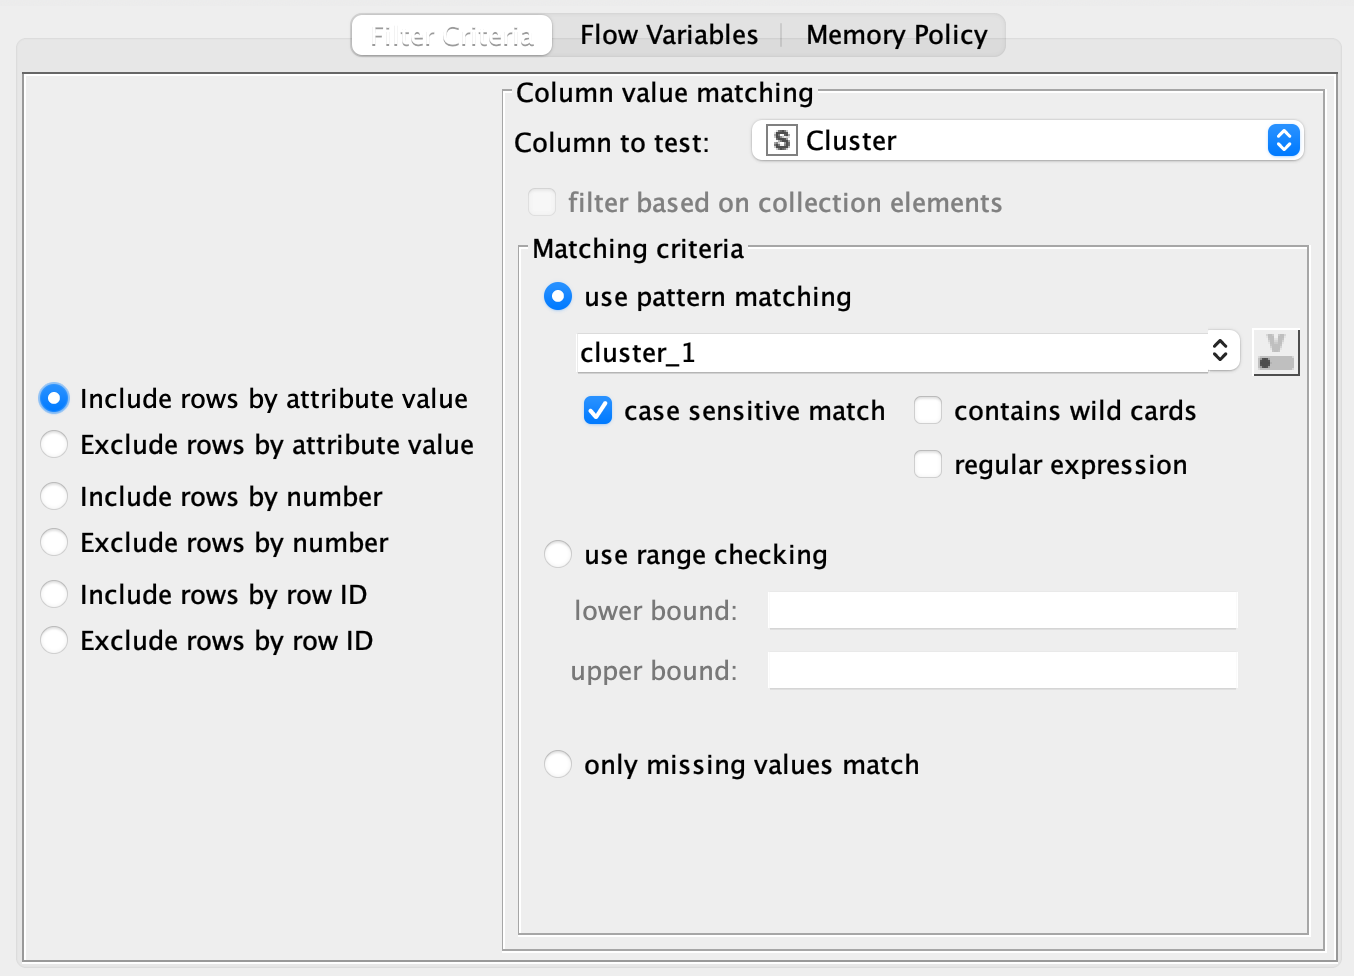
\includegraphics[width=\textwidth]{res/t1/t14/t14-row-filter-2-conf}
					\caption{Color Manager}
					\label{fig:second}
				\end{subfigure}
				\hfill
				\begin{subfigure}{0.4\textwidth}
					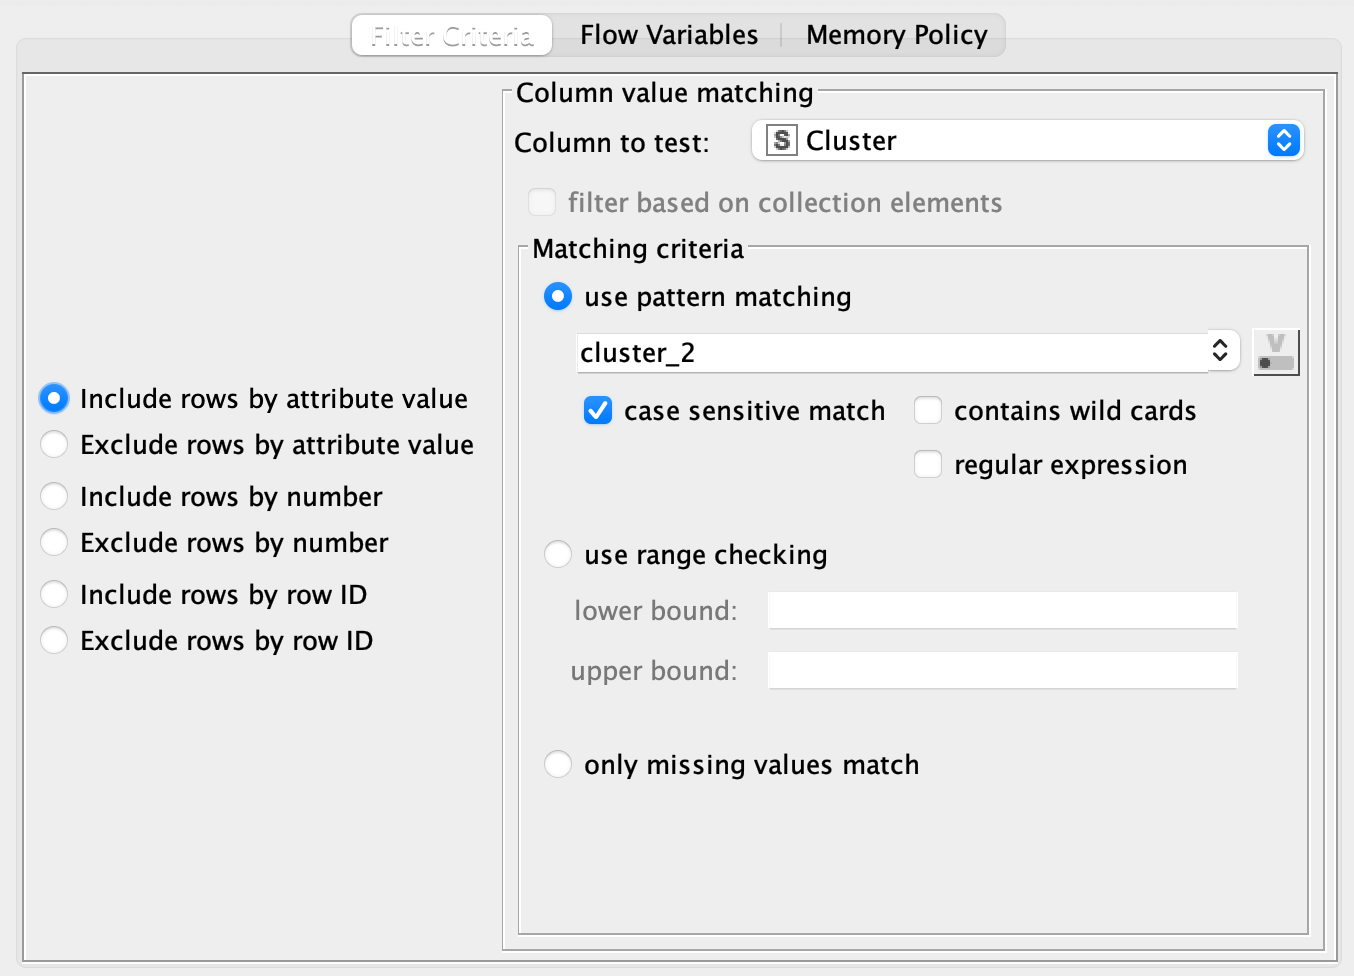
\includegraphics[width=\textwidth]{res/t1/t14/t14-row-filter-3-conf}
					\caption{Duplicate Row Filter}
					\label{fig:third}
				\end{subfigure}	
				\label{fig:figures}
			\end{figure}
			\fi
			\subsubsection*{Prerequisite 1 : Sum of Square Estimate of Errors(SSE)}
				Before our attempt of explaining WSS and BSS, it is essential to explain SSE (Sum of Square estimate of Errors). SSE is an evaluation metric with a plethora of applications in statistics and predictive analytics\cite{???}. It is used to evaluate a model's performance against a training set\cite{???}. The logic behind SSE is rather simple in nature. Let X an random variable and a model $y=\bar{X}$
				\iftrue
				\begin{center}
					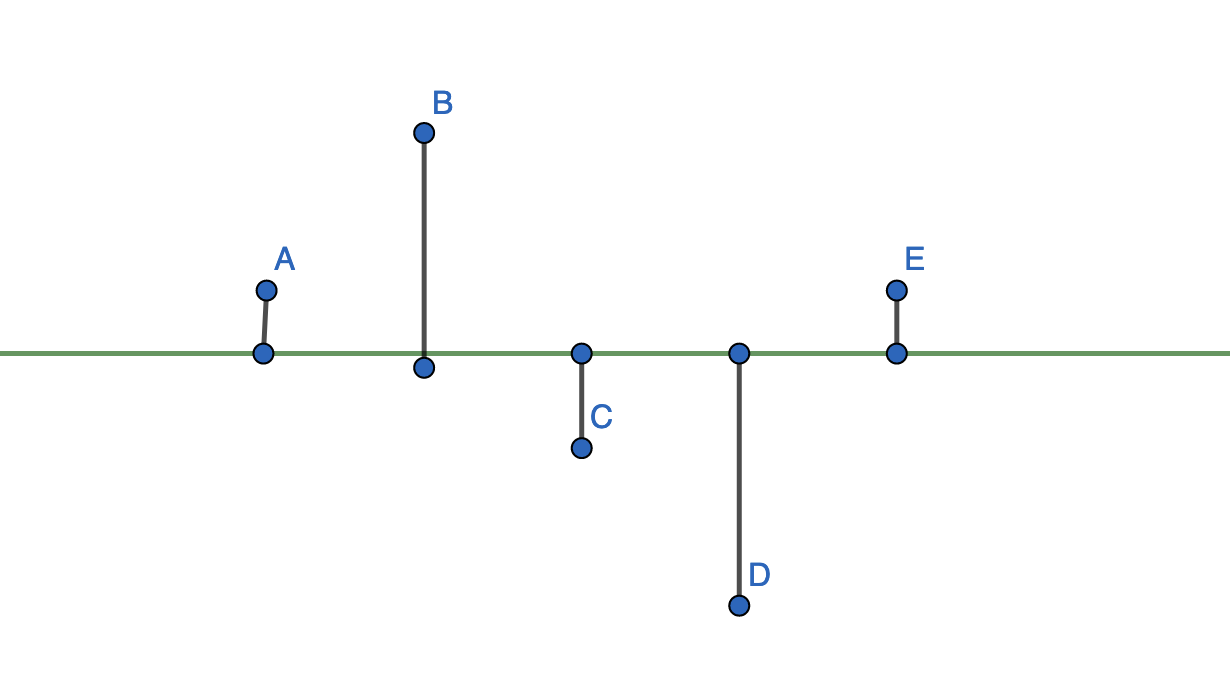
\includegraphics[scale=0.5]{res/task-1/SSE-1}				
				\end{center}
				\fi
				We can evaluate our model's performance, by calculating the Sum of Errors, where 'error' in this case, is the distance of the observed variable from the responce of our model (i.e the mean $\bar{X}$), as follows
				\iftrue
				\begin{align}
					SE = \sum_{i=1}^{n}{X_i-\bar{X}}
				\end{align}
				\fi
				Unfortunately, our evaluation metric has a fatal flaw, it allows for error's to 'cancel out' simply because they are placed beneath our model's line. It can be proven that, for the case of $y=\bar{X}$ SE is always 0.
				\iftrue
				\begin{align}
					SE = \sum_{i=1}^{n}{X_i-\bar{X}} \\
					SE = \sum_{i=1}^{n}{X_i} - \sum_{i=1}{n}{\bar{X}} \\
					SE = \sum_{i=1}^{n}{X_i} - n\bar{X} \\
					SE = \sum_{i=1}^{n}{X_i} - \sum_{i=1}^{n}{X_i} \\
					SE = 0 \\
				\end{align}
				\fi
				For other models(in higher dimensions, where corellation of the involved variables is not 1), it may not be zero, but the fatal flaw remains, by cancelling errors we severely underestimate the errors involved. A more appropriate approach could be to square the distances, that would give us the Sum of Squared Errors (SSE)\\
				\iftrue
				\begin{align}
					SE = \sum_{i=1}^{n}{(X_i-\bar{X})}^2
				\end{align}
				\fi
			\subsubsection*{WSS and BSS}
				In the world of Clustering models performance evaluation, SSE is translated into two distinct but related ideas\cite{???}, WSS and BSS
				\iftrue
				\begin{figure}[H]
					\centering
					\begin{subfigure}{0.4\textwidth}
						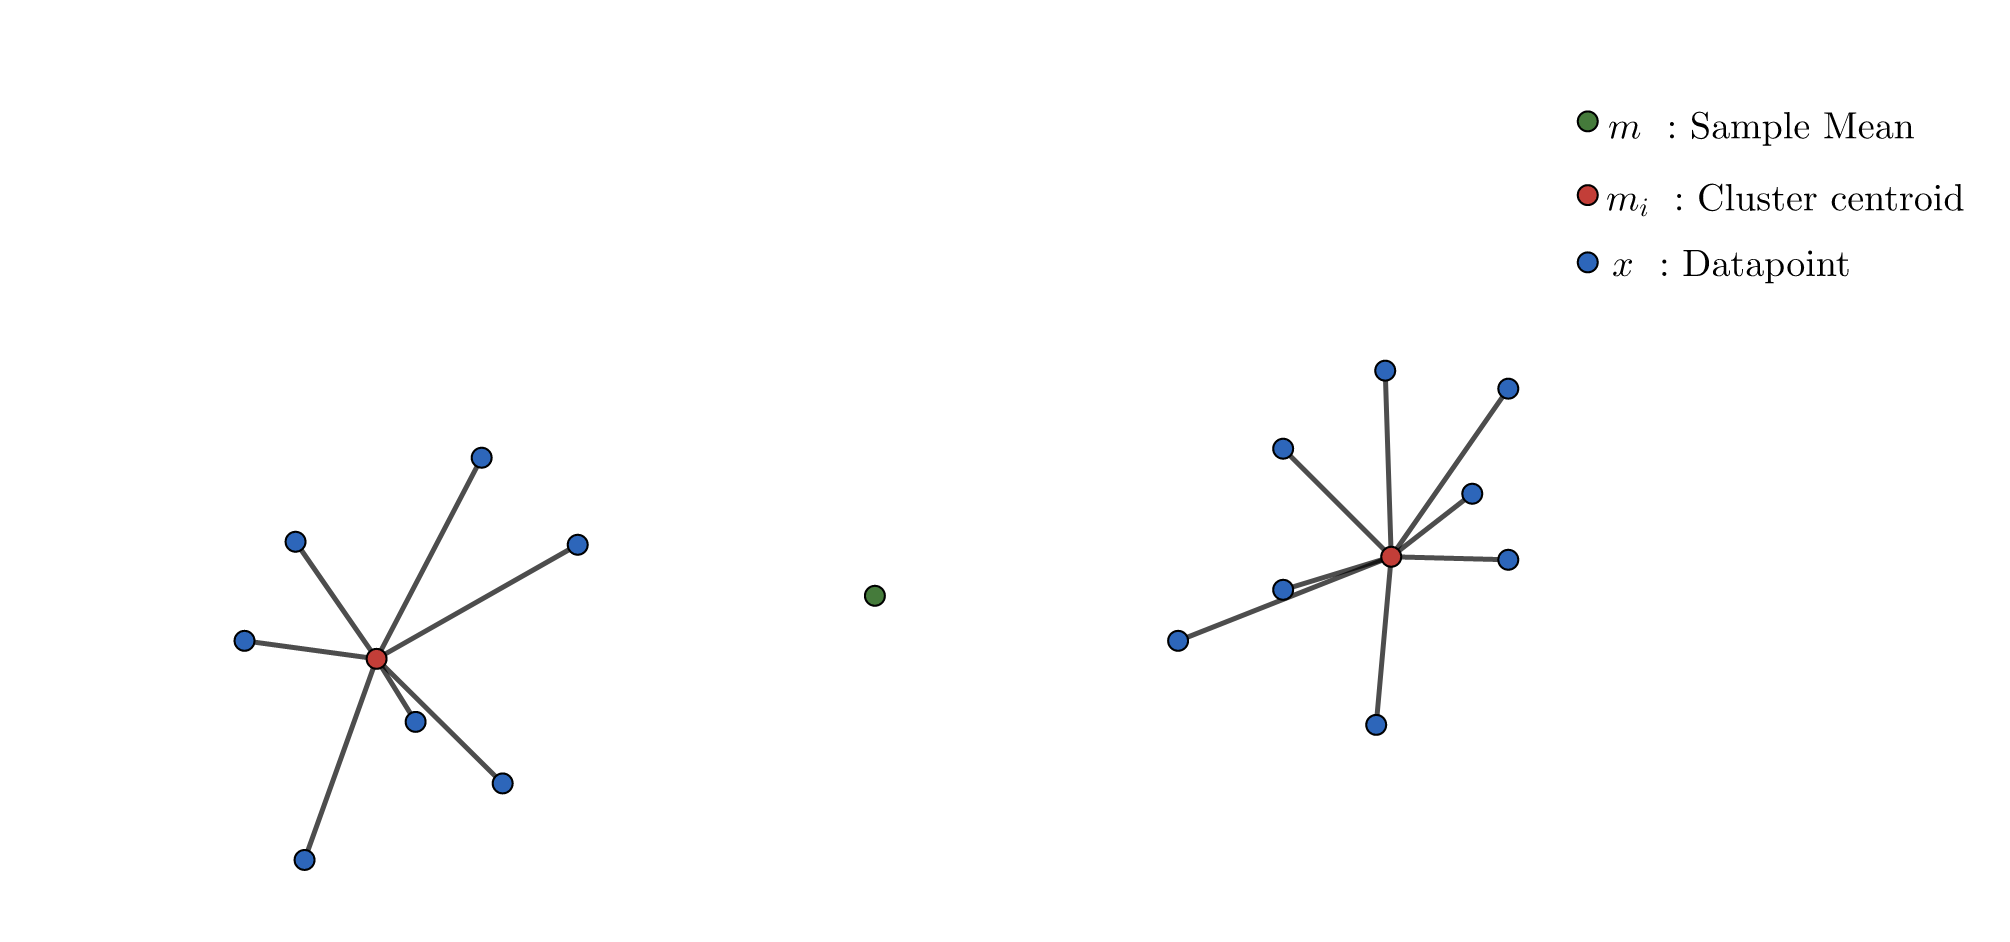
\includegraphics[width=\textwidth]{res/task-1/WSS}
						\caption{WSS}
						\label{fig:first}
					\end{subfigure}
					\hfill
					\begin{subfigure}{0.4\textwidth}
						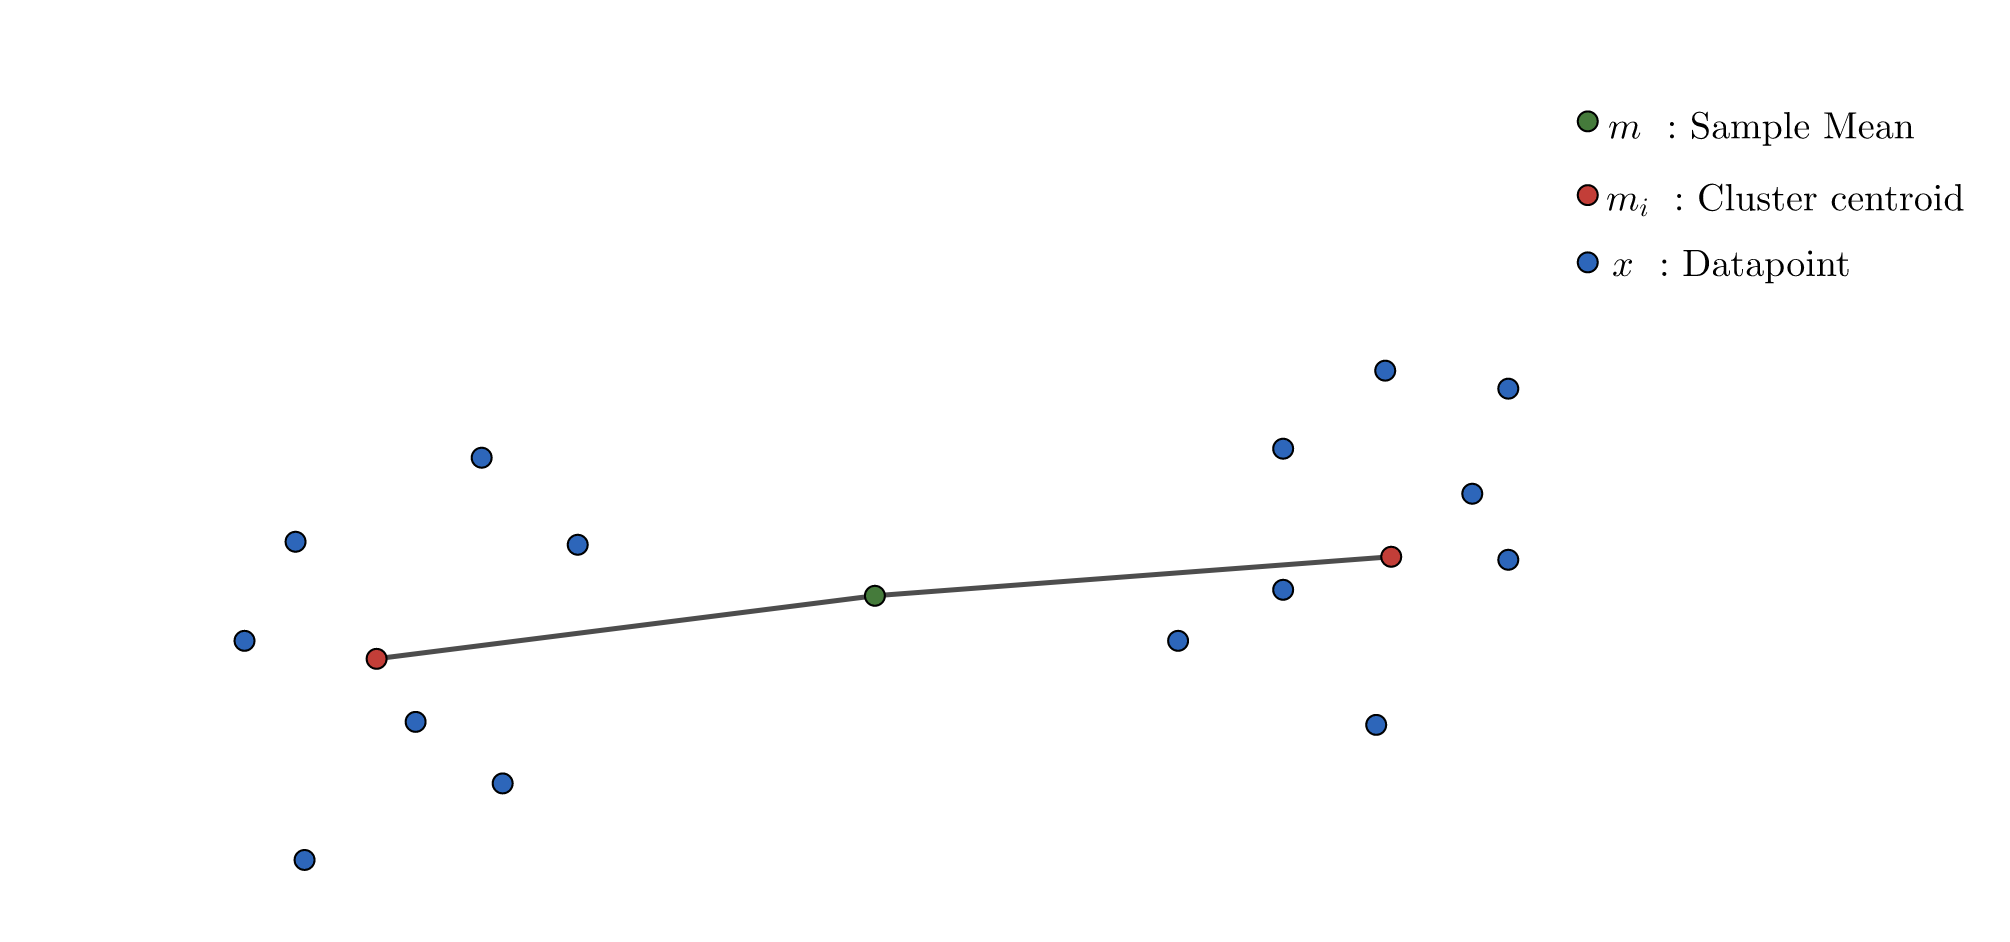
\includegraphics[width=\textwidth]{res/task-1/BSS}
						\caption{BSS}
						\label{fig:second}
					\end{subfigure}
					\hfill
					\label{fig:figures}
				\end{figure}
				\fi
			\subsubsection*{WSS}
				WSS or  Within Cluster Sum of Squares is a clustering model performance evaluation function. Our 'model' in this case is the cluster centroid and the error is the distance for each datapoint from the cluster centroid. WSS can be evaluated with the following formula\cite{???}
				\iftrue
				\begin{align}
					WSS = \sum_{i=1}^{k}{\sum_{x\in{C_i}}^{}{(x-m_i)^2}}	
				\end{align}
				\fi
				Where $k$, the number of clusters involved, $C_i$ the individual cluster and $m_i$, the given cluster centroid.
				\subsubsection*{BSS}
				BSS or  Between Cluster Sum of Squares is a clustering model performance evaluation function, just like WSS. Our 'model' in this case is the overall data mean and the error is the distance of each cluster's centroid to the overall mean. BSS can be evaluated with the following formula\cite{???}
				\iftrue
				\begin{align}
					BSS = \sum_{i=1}^{k}{\abs{C_i}(m-m_i)^2}	
				\end{align}
				\fi
				Where $k$, the number of clusters involved, $C_i$ the individual cluster and $m_i$, the given cluster centroid.
			\subsubsection*{Interpretation}
				A good clustering solution, would involve well separated clusters, with low WSS to BSS ratio\cite{???}. As K-Means is a heuristic based algorithm, we will not analyse WSS and BSS of a single K-Means run, but rather we will analyse their behaviour after a sequence of 100 runs. 
				\iftrue
				\begin{figure}[H]
					
					\centering
					\begin{subfigure}{0.4\textwidth}
						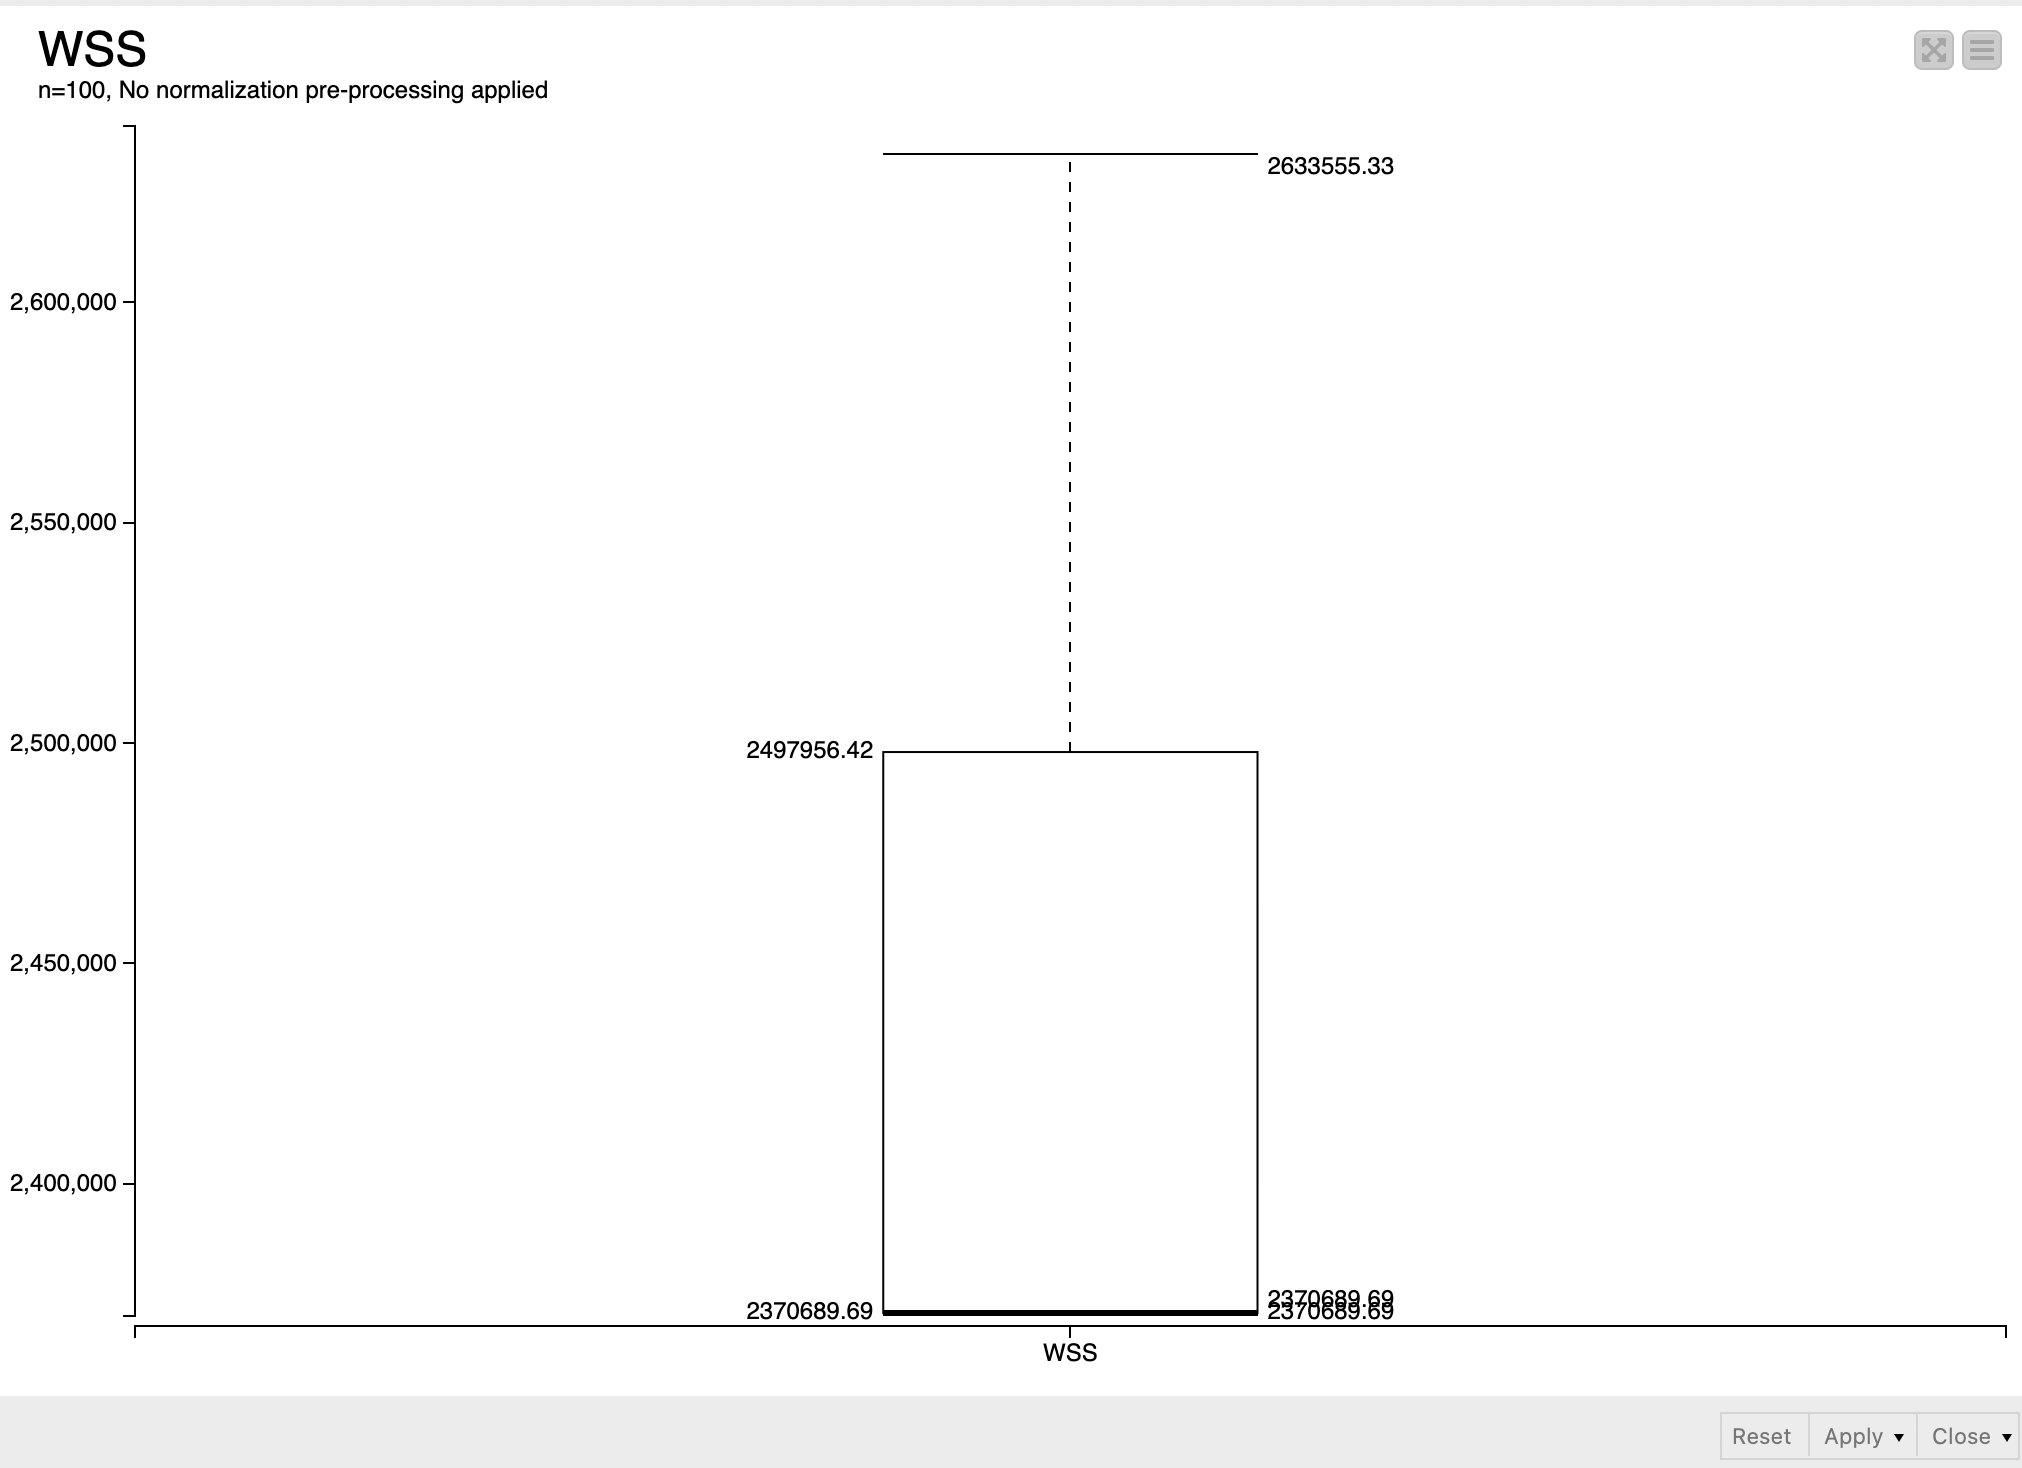
\includegraphics[width=\textwidth]{res/task-1/WSS-Knime}
						\caption{WSS}
						\label{fig:first}
					\end{subfigure}
					\hfill
					\begin{subfigure}{0.4\textwidth}
						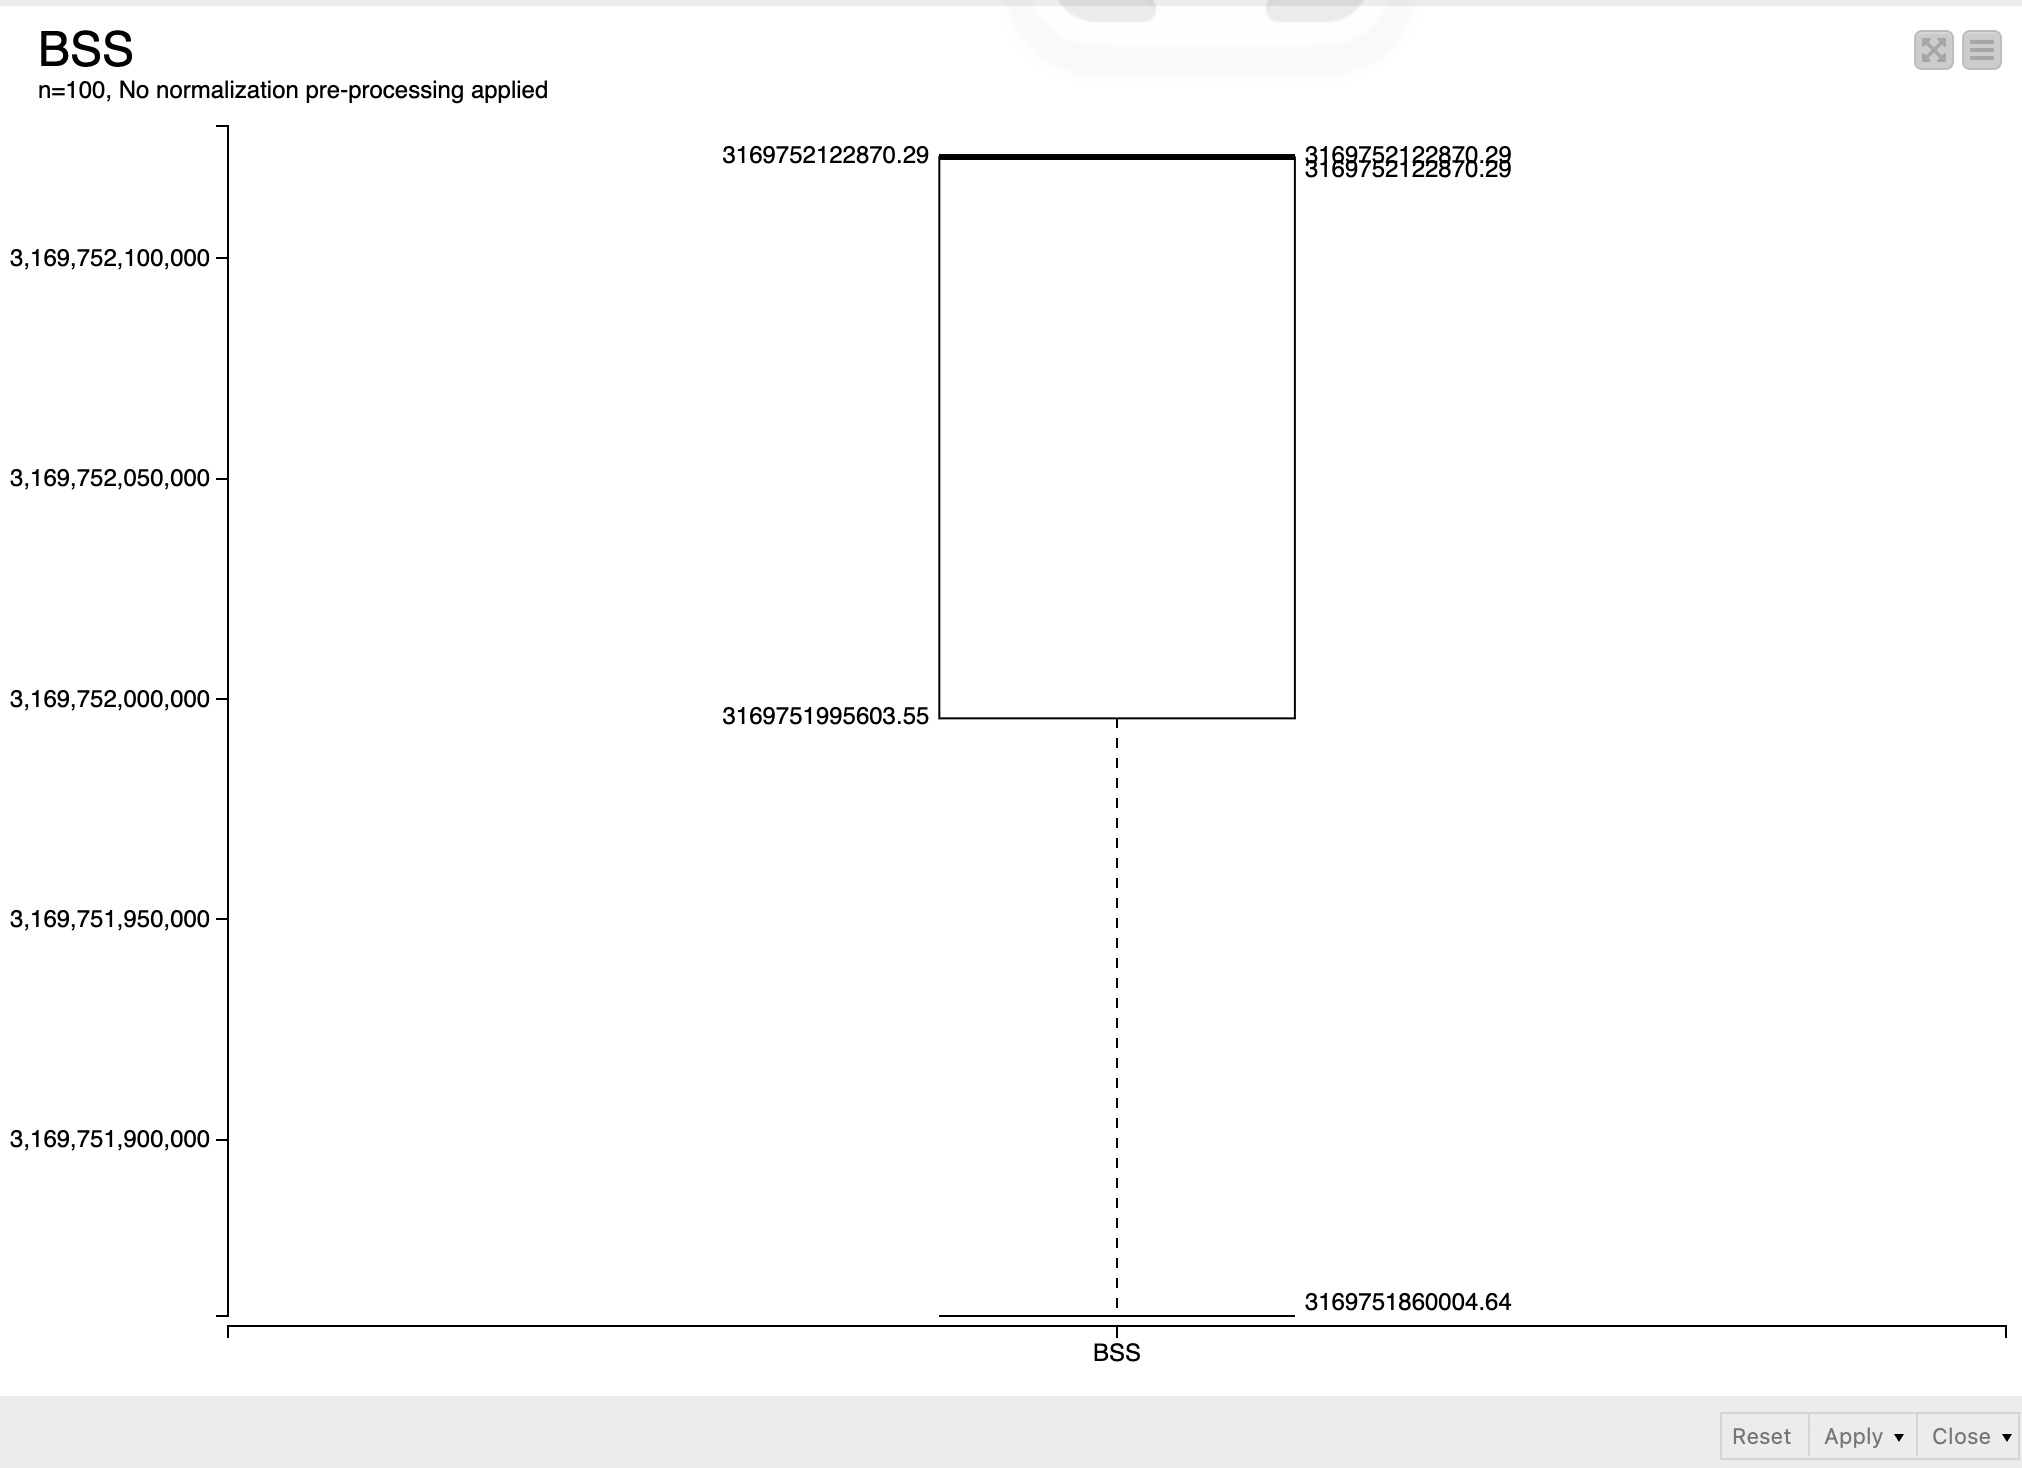
\includegraphics[width=\textwidth]{res/task-1/BSS-Knime}
						\caption{BSS}
						\label{fig:second}
					\end{subfigure}
					\hfill
					\begin{subfigure}{0.4\textwidth}
						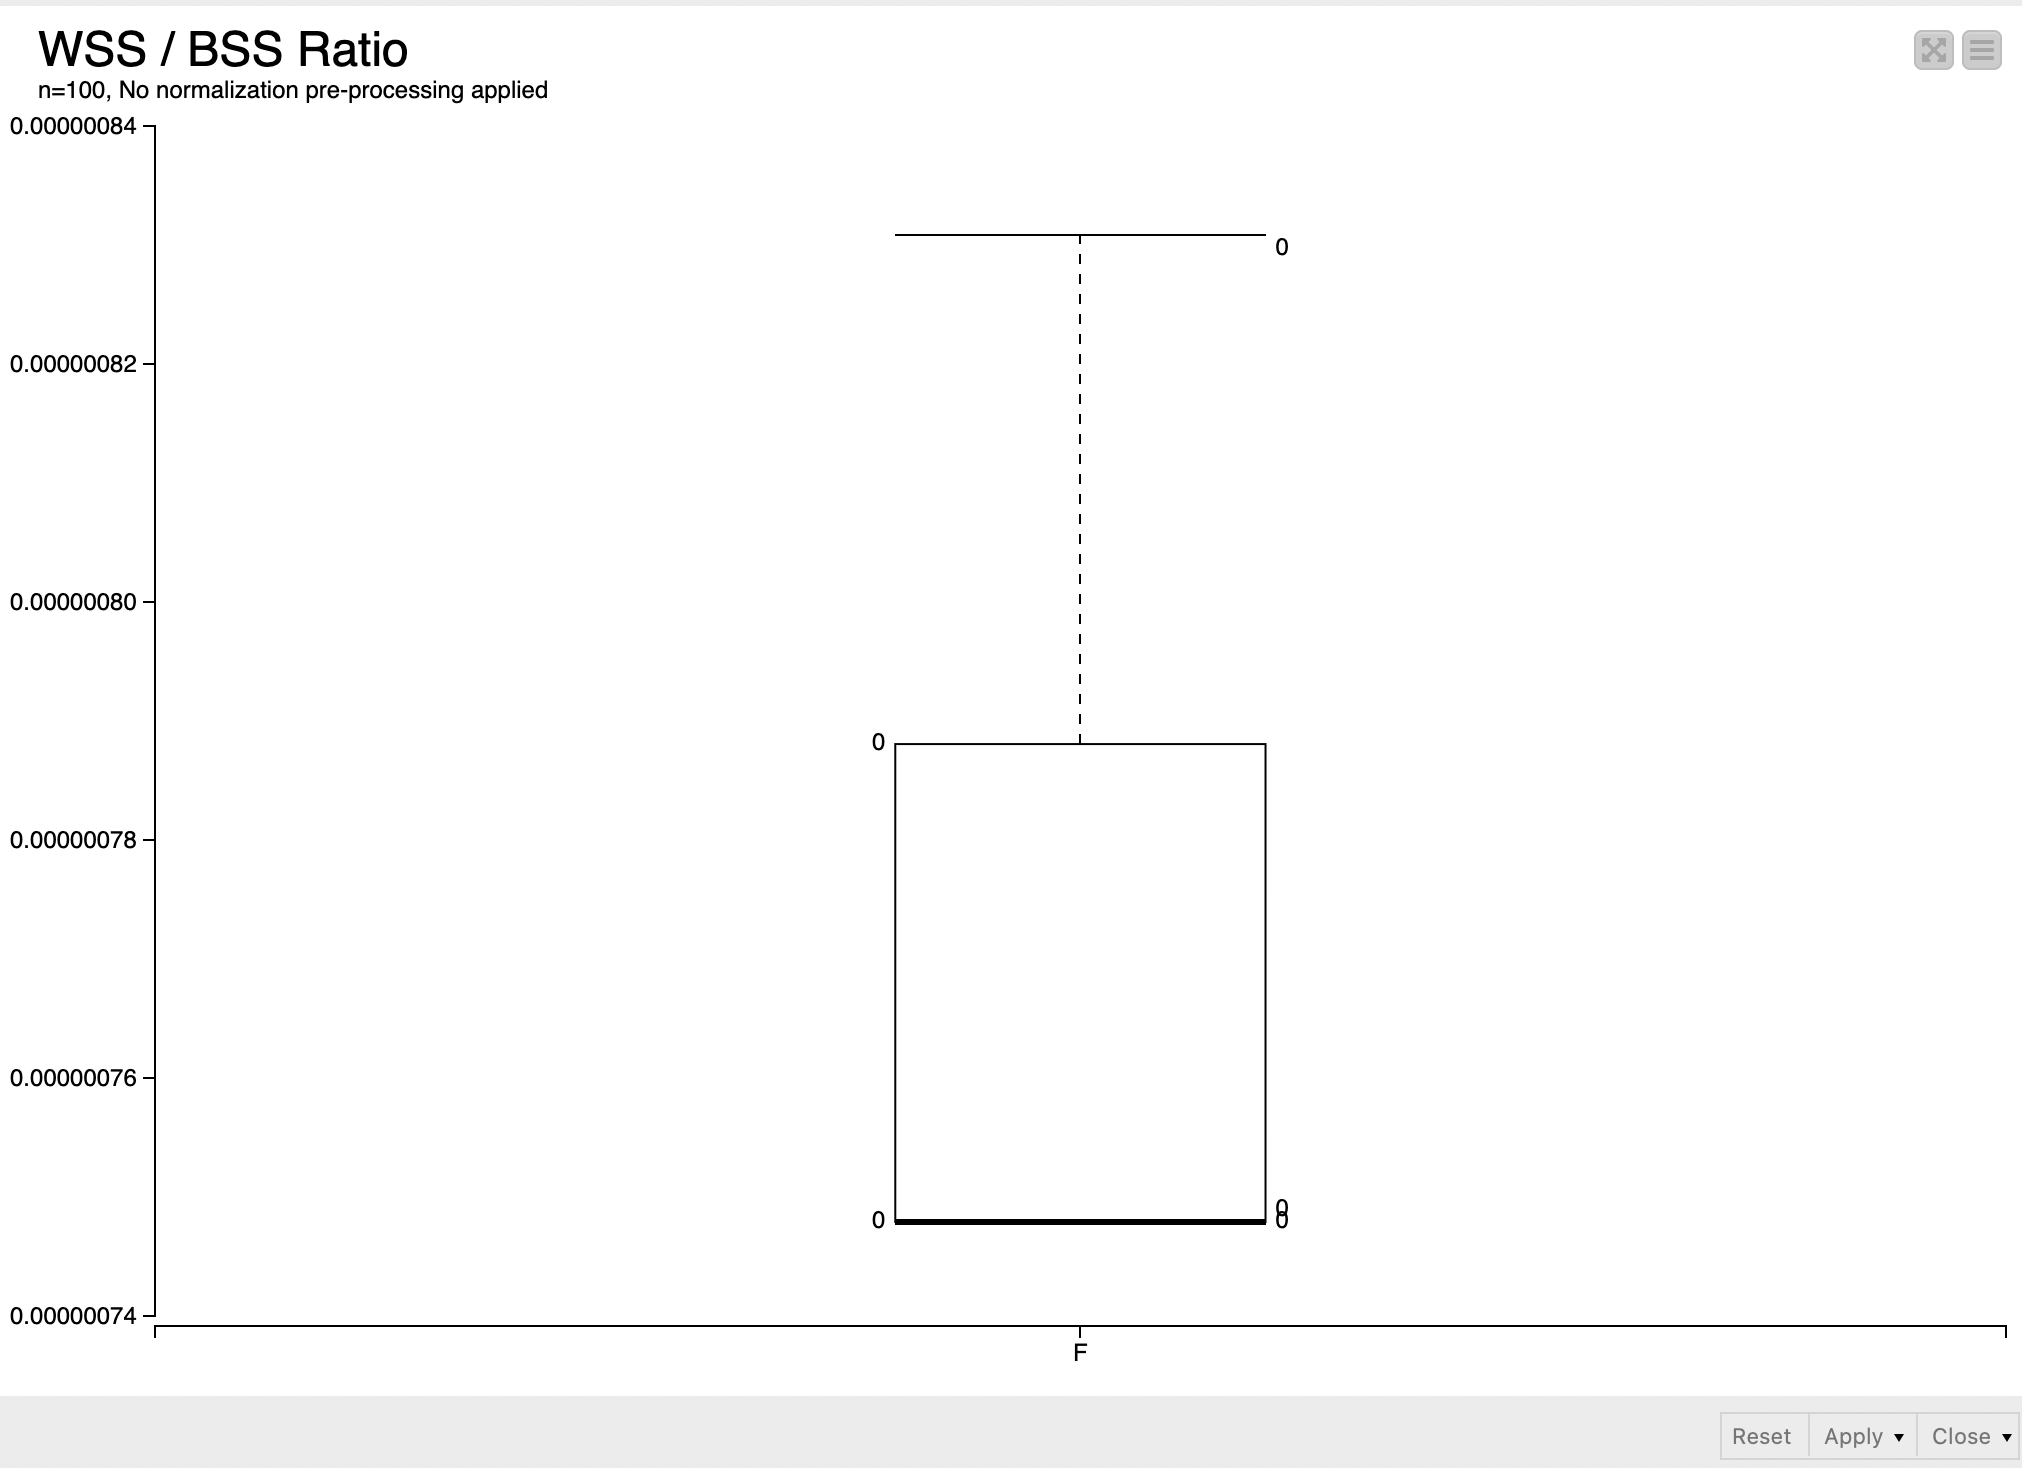
\includegraphics[width=\textwidth]{res/task-1/WSS-BSS-Ratio}
						\caption{Ratio}
						\label{fig:third}
					\end{subfigure}
					\label{fig:figures}	
				\end{figure}
				\fi
				As we can see, The ratio of WSS to BSS is very small, something that indicates well separated clusters(i.e a good clustering solution). However, a single cluster validity measure on its own, is insufficient to provide enough evidence for a meaningful clustering. Taking into consideration our observations from Task 1.3 and Task 1.4, this clustering \cite{???}is not meaningful, is full of
				errors, mainly due to the absence of the normalisation pre-processing step.
	\section*{Task 2}
		\subsection*{The Importance of Normalisation}
			The standard Lorem Ipsum passage, used since the 1500s
			
			"Lorem ipsum dolor sit amet, consectetur adipiscing elit, sed do eiusmod tempor incididunt ut labore et dolore magna aliqua. Ut enim ad minim veniam, quis nostrud exercitation ullamco laboris nisi ut aliquip ex ea commodo consequat. Duis aute irure dolor in reprehenderit in voluptate velit esse cillum dolore eu fugiat nulla pariatur. Excepteur sint occaecat cupidatat non proident, sunt in culpa qui officia deserunt mollit anim id est laborum."
			Section 1.10.32 of "de Finibus Bonorum et Malorum", written by Cicero in 45 BC
		\subsection*{The Inner-workings of normalisation}
			The standard Lorem Ipsum passage, used since the 1500s
			
			"Lorem ipsum dolor sit amet, consectetur adipiscing elit, sed do eiusmod tempor incididunt ut labore et dolore magna aliqua. Ut enim ad minim veniam, quis nostrud exercitation ullamco laboris nisi ut aliquip ex ea commodo consequat. Duis aute irure dolor in reprehenderit in voluptate velit esse cillum dolore eu fugiat nulla pariatur. Excepteur sint occaecat cupidatat non proident, sunt in culpa qui officia deserunt mollit anim id est laborum."
			Section 1.10.32 of "de Finibus Bonorum et Malorum", written by Cicero in 45 BC
		\subsection*{Changes in the workflows}
			The standard Lorem Ipsum passage, used since the 1500s
			
			"Lorem ipsum dolor sit amet, consectetur adipiscing elit, sed do eiusmod tempor incididunt ut labore et dolore magna aliqua. Ut enim ad minim veniam, quis nostrud exercitation ullamco laboris nisi ut aliquip ex ea commodo consequat. Duis aute irure dolor in reprehenderit in voluptate velit esse cillum dolore eu fugiat nulla pariatur. Excepteur sint occaecat cupidatat non proident, sunt in culpa qui officia deserunt mollit anim id est laborum."
			Section 1.10.32 of "de Finibus Bonorum et Malorum", written by Cicero in 45 BC
		\subsection*{New Plots}
			The standard Lorem Ipsum passage, used since the 1500s
			
			"Lorem ipsum dolor sit amet, consectetur adipiscing elit, sed do eiusmod tempor incididunt ut labore et dolore magna aliqua. Ut enim ad minim veniam, quis nostrud exercitation ullamco laboris nisi ut aliquip ex ea commodo consequat. Duis aute irure dolor in reprehenderit in voluptate velit esse cillum dolore eu fugiat nulla pariatur. Excepteur sint occaecat cupidatat non proident, sunt in culpa qui officia deserunt mollit anim id est laborum."
			Section 1.10.32 of "de Finibus Bonorum et Malorum", written by Cicero in 45 BC
		\subsection*{Compare and Contrast}
			The standard Lorem Ipsum passage, used since the 1500s
			
			"Lorem ipsum dolor sit amet, consectetur adipiscing elit, sed do eiusmod tempor incididunt ut labore et dolore magna aliqua. Ut enim ad minim veniam, quis nostrud exercitation ullamco laboris nisi ut aliquip ex ea commodo consequat. Duis aute irure dolor in reprehenderit in voluptate velit esse cillum dolore eu fugiat nulla pariatur. Excepteur sint occaecat cupidatat non proident, sunt in culpa qui officia deserunt mollit anim id est laborum."
			Section 1.10.32 of "de Finibus Bonorum et Malorum", written by Cicero in 45 BC
		
		 
		
	
	\pagebreak
	\begin{thebibliography}{1}	
		\bibitem{entropy}
		\textit{Shannon, C., 1948. A Mathematical Theory of Communication. Bell System Technical Journal, 27(3), pp.379-423.}
		
	\end{thebibliography}
\end{document}
